\documentclass[eind]{penoverslag}

%%% PACKAGES
\usepackage{lipsum}
\usepackage{gensymb}
\usepackage [dutch] {babel}
\usepackage{graphicx}
\usepackage{amsmath}
\usepackage{listings}
\usepackage{caption}
\usepackage{subcaption}
\usepackage{tikz}
\usetikzlibrary{shapes,shadows,arrows}
\usepackage{tocloft} %sets dots in the TOC after the sections
	\renewcommand{\cftsecleader}{\cftdotfill{\cftdotsep}}
\usepackage[absolute]{textpos}
	\setlength{\TPHorizModule}{1cm}
	\setlength{\TPVertModule}{1cm}
\usepackage{enumitem} %witruimte voor lijstjes
	\setitemize{noitemsep,topsep=0pt,parsep=3pt,partopsep=5pt}
	\setenumerate{noitemsep,topsep=0pt,parsep=5pt,partopsep=10pt}

\begin{document}

\team{Zilver} % teamkleur
\members{Sam Gielis\\
         Sophie Marien\\
         Toon Nolten\\
         Nele Rober\\
         Gerlinde Van Roey\\
         Maxim Van Mechelen} % teamleden

\maketitlepage

\newpage
%TODO De Doolhof en Het Doolhof nakijken voor consequente schrijfwijze. Gekalibreerd en gecalibreerd

\begin{abstract}
\label{ssec:Abstract}
Het P\&O-project heeft als doel vier autonome robots \textit{Team Treasure Trek} \cite{TeamTreasure} te laten spelen. Dit verslag beschrijft de invulling die team Zilver aan het project gaf.\\

De robot is voorzien van een lichtsensor, een infraroodsensor en een ultrasone sensor. Verder heeft de robot een lange schep waarmee hij zijn voorwerp kan oprapen en eventueel een wip kan openen.
De robot kan een doolhof verkennen en hiervan een kaart (verder een `map' genoemd) bijhouden. Andere robots worden vermeden met behulp van de ultrasone sensor. Via \textsc{RabbitMQ} \cite{RabbitMQ} kunnen de robots elkaars mappen en posities doorsturen. Door zijn eigen map samen te voegen met die van zijn teamgenoot, kan de robot een pad tot bij zijn teamgenoot bepalen.\\

Het computerprogramma simuleert de werking van de robot. Deze simulator kan in combinatie met de fysieke robot gebruikt worden en kan meerdere robots tegelijkertijd simuleren. De gesimuleerde robots gedragen zich volledig analoog aan de fysieke robot.
\end{abstract}

%figuur robot
\begin{figure}[!hb]
\begin{textblock}{38}(5,11)
    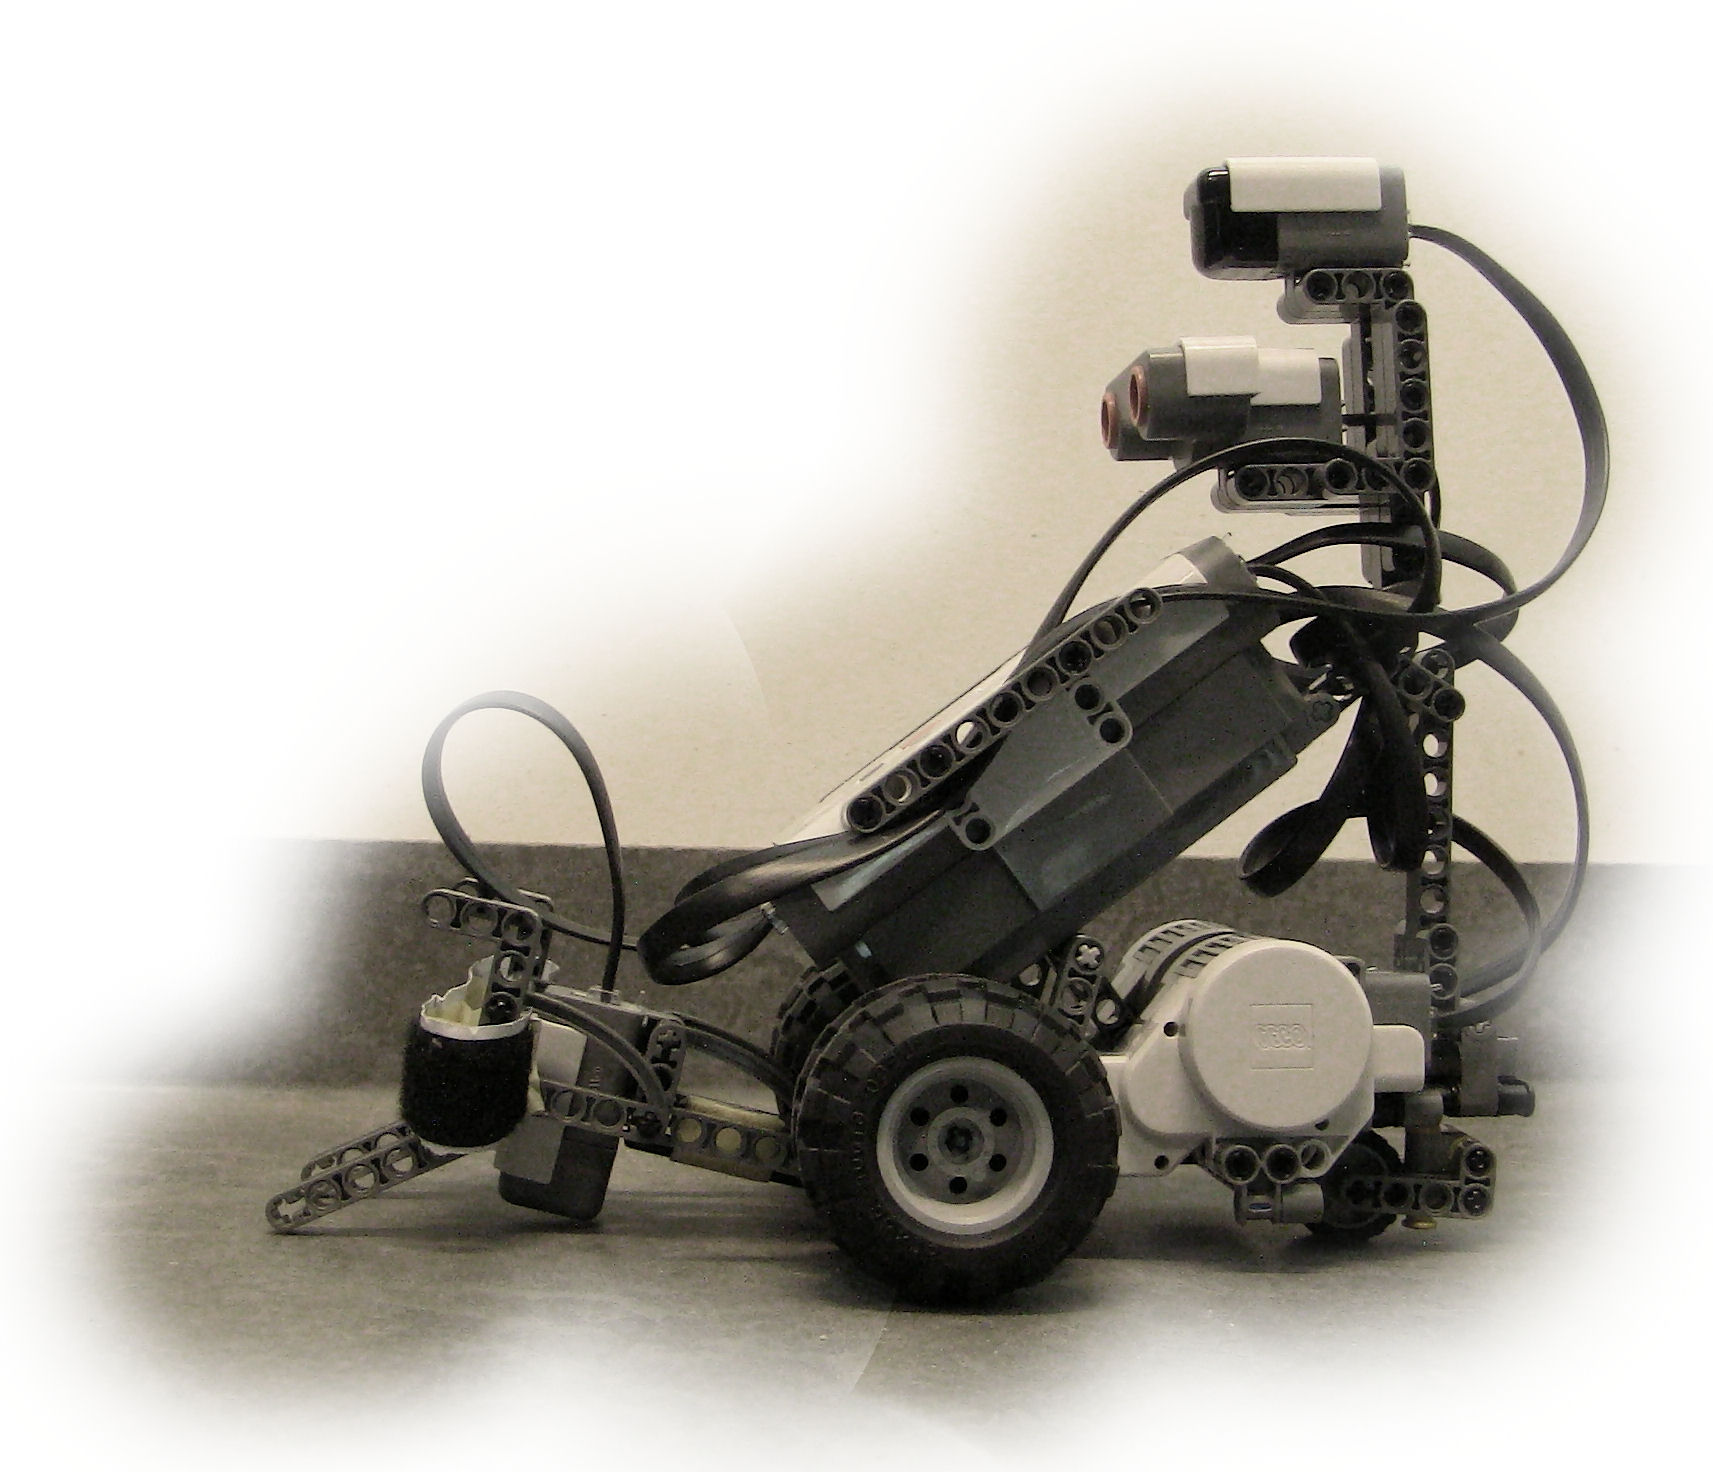
\includegraphics[width=0.40\textwidth]{robotFP}
    \label{fig:robotFP}
\end{textblock}
\end{figure}

\newpage
\setcounter{tocdepth}{3}
\tableofcontents
\newpage

% == INLEIDING == %
\section{Inleiding} % 4 ok
\label{ssec:Inl}
In het kader van het vak `Probleemoplossen en Ontwerpen: Computerwetenschappen' wordt gewerkt rond autonome intelligente robots. Verschillende teams bouwen en programmeren een robot met behulp van \textsc{LEGO Mindstorms} \cite{mindstorms}. Deze robot moet uiteindelijk samen met drie andere robots volledig autonoom \textit{Team Treasure Trek} kunnen spelen.
De robots moeten hierbij in een onbekend doolhof op zoek gaan naar het voorwerp dat hen toegewezen werd. Wanneer een robot zijn voorwerp gevonden heeft, komt hij te weten met welke robot hij moet samenwerken. Elk duo moet beide voorwerpen bij elkaar brengen. Het duo dat hier eerst in slaagt, wint.\\

Een doolhof bestaat uit houten tegels van~$40$ op $40$~cm. De rand van een tegel wordt aangegeven door een witte lijn of een opstaande muur. Tegels kunnen een barcode bevatten die uit witte en zwarte lijnen bestaat. Een doolhof bevat mogelijk een wip: vier tegels die kantelen wanneer de robot erover rijdt. Onder een wip wordt een bal geplaatst die infrarood licht uitzendt. Het is uiteraard enkel mogelijk een wip op te rijden wanneer deze naar beneden staat.

Als voorwerp wordt een wc-rol gebruikt.\\

De fysieke bouw van de robot en de kalibratie van de sensoren wordt beschreven in sectie~\ref{sec:Robot}. Algoritmes die toelaten de verschillende aspecten van het spel te spelen worden beschreven in sectie~\ref{sec:Algo}. Ten slotte wordt in sectie~\ref{sec:Softw} een overzicht gegeven van de verschillende softwareonderdelen en hun onderlinge relaties.

\section{Robot}
\label{sec:Robot}
\textsc{LEGO Mindstorms} biedt een bouwpakket voor een robot aan. Het pakket bevat een \textsc{NXT}-microcomputer die toelaat de robot te programmeren. Met behulp van \textsc{leJOS} \cite{leJOS} kan dit in \textsc{Java}. Sectie~\ref{ssec:Bouw} beschrijft de bouw van de robot, sectie~\ref{ssec:Kalib} de kalibratie van de motoren en de sensoren.

\subsection{Bouw Robot}
\label{ssec:Bouw}
Bovenaan de robot staat een infrarood- en ultrasone sensor gemonteerd. Deze kunnen niet bewegen ten opzichte van de robot. De lichtsensor werd op een scharnier gemonteerd, zodat deze omhoog kantelt wanneer hij een wip raakt. Dit zorgt ervoor dat de robot vlot de wip op kan. De sensoren worden weergegeven in figuur~\ref{fig:robotDetail}.\\

Een voorwerp is voorzien van klittenband en kan op verschillende manieren worden opgeraapt. Volgende opstellingen werden gebouwd en getest:

\begin{enumerate}
\item \textbf{Figuur~\ref{fig:robotOud1} } De robot heft het voorwerp op met behulp van een schep achteraan. De schep is voorzien van een extra motor. Deze opstelling maakt de robot echter te lang waardoor hij moeilijker kan draaien zonder tegen een muur te botsen;
\item \textbf{Figuur~\ref{fig:robotOud2} } De schep wordt vooraan geplaatst, waar te weinig plaats is voor een extra motor. De schep aanpassen aan de vorm van het voorwerp blijkt echter niet voldoende om het voorwerp succesvol op te rapen;
\item \textbf{Figuur~\ref{fig:robotOud3} } Klittenband zorgt ervoor dat het voorwerp beter in de schep blijft liggen. Deze opstelling maakt de robot echter nog steeds te lang;
\item \textbf{Figuur~\ref{fig:robotBouw} } Door de \textsc{NXT} horizontaal te plaatsen en de extra motor tussen de wielen te monteren, wordt de robot compacter. De bredere basis maakt de robot bovendien stabieler. Een lange schep met klittenband achteraan laat toe het voorwerp op te rapen en eventueel een wip te openen.
\end{enumerate}

Deze laatste opstelling gaf voorlopig nog geen problemen. Dit is de huidige opstelling. Figuur~\ref{fig:robotDetail} toont details van de schep en de sensoren.

% bouw robot: oude ontwerpen
\begin{figure}
\centering
	\begin{subfigure}[h]{0.325\textwidth}
	\centering
		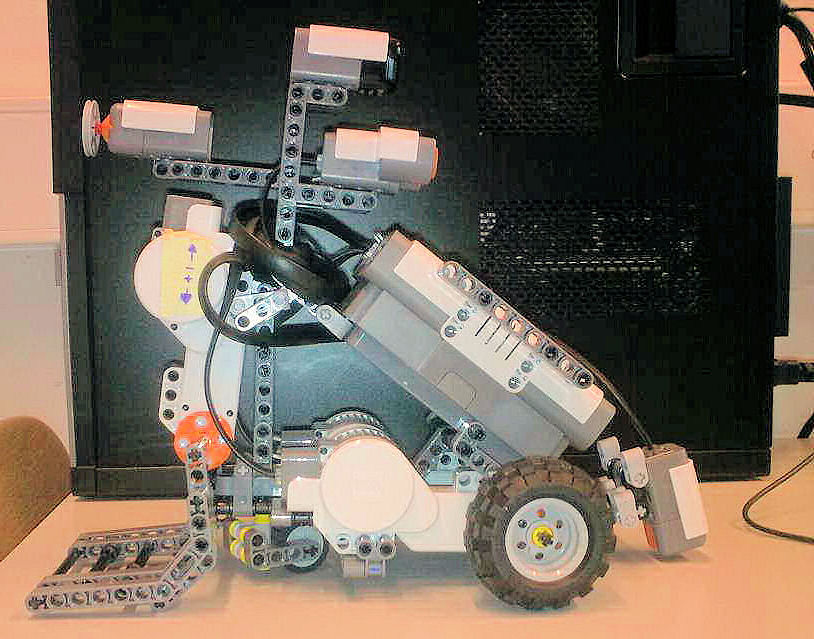
\includegraphics[width=\textwidth]{robotOud1}
		\caption{Schep achteraan}
		\label{fig:robotOud1}
	\end{subfigure}
	\begin{subfigure}[h]{0.325\textwidth}
		\centering
		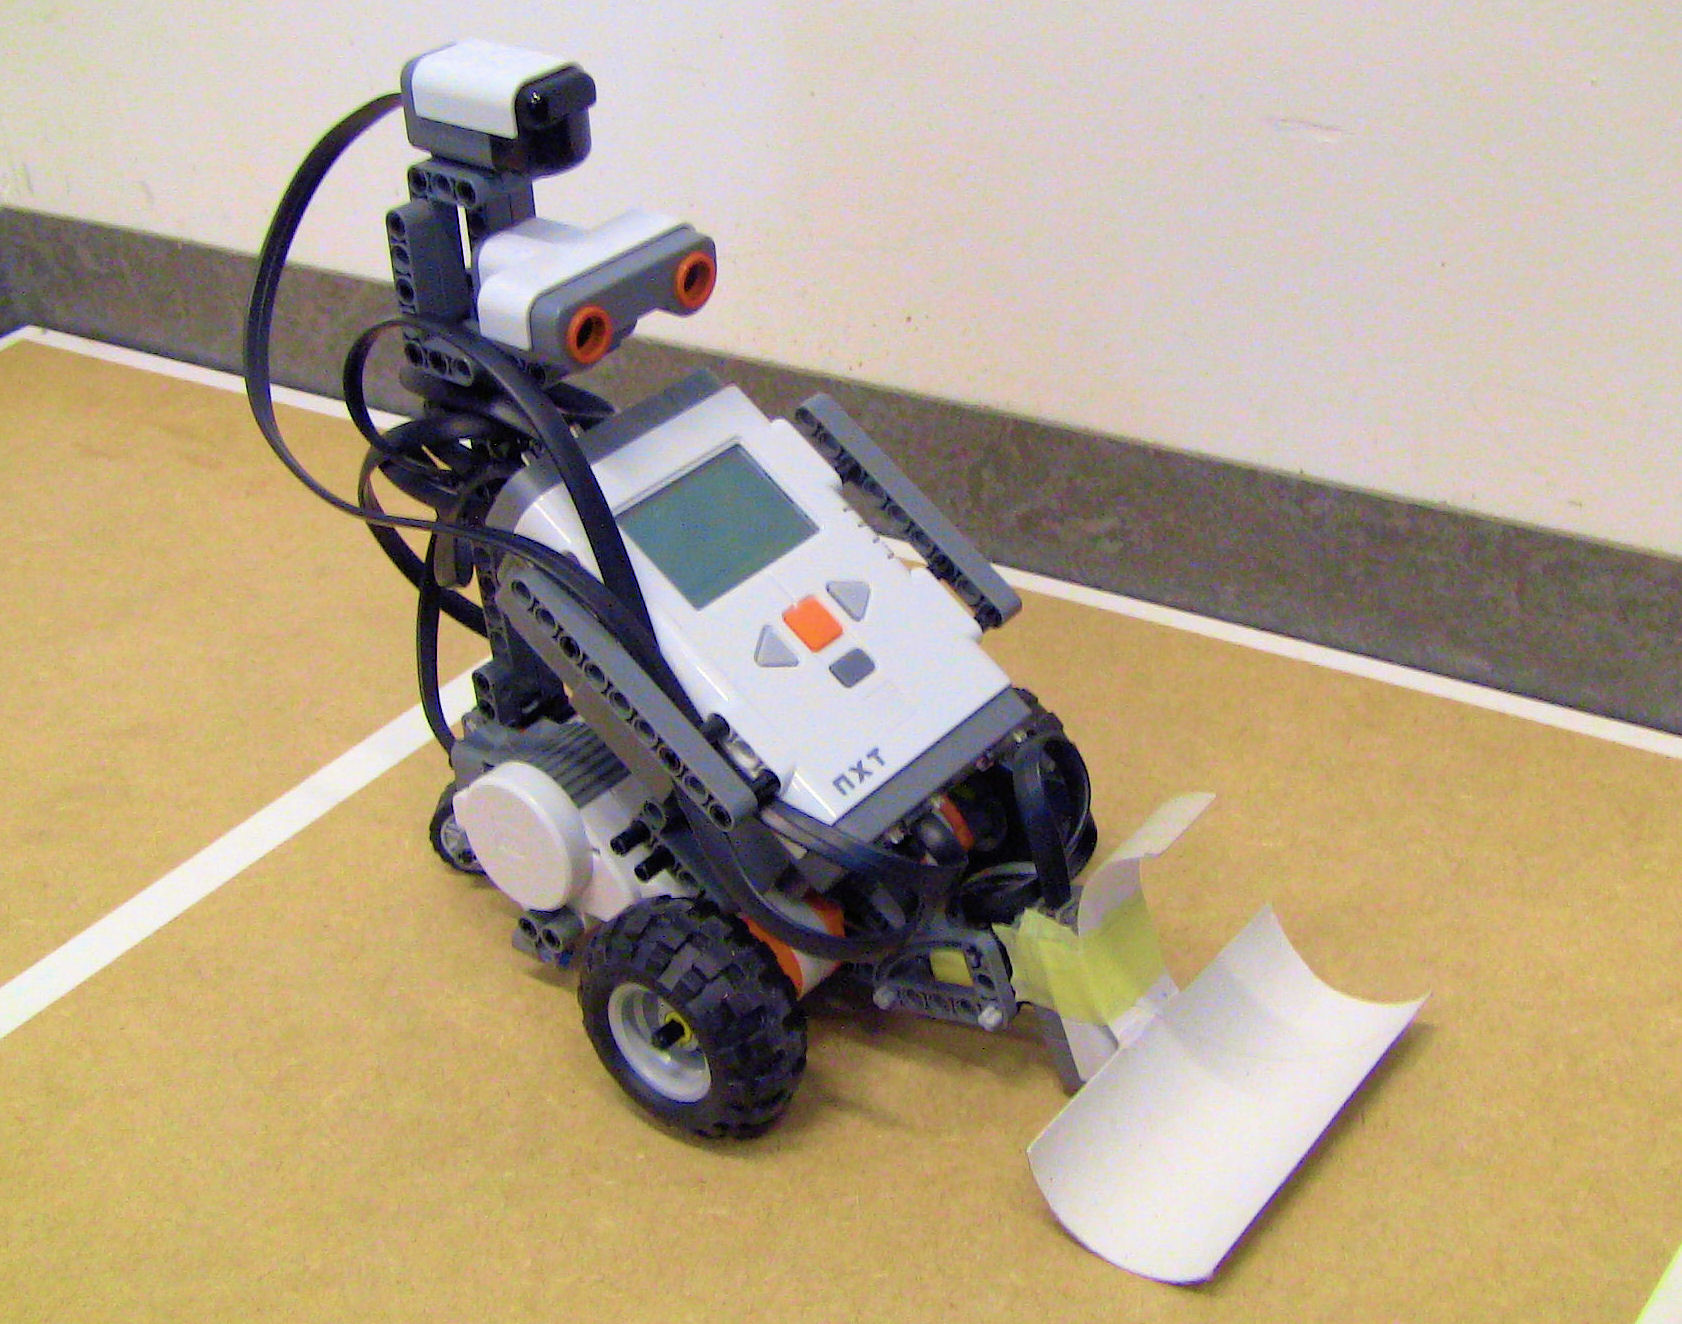
\includegraphics[width=\textwidth]{robotOud2}
		\caption{Kartonnen schep vooraan}
		\label{fig:robotOud2}
	\end{subfigure}
	\begin{subfigure}[h]{0.325\textwidth}
		\centering
		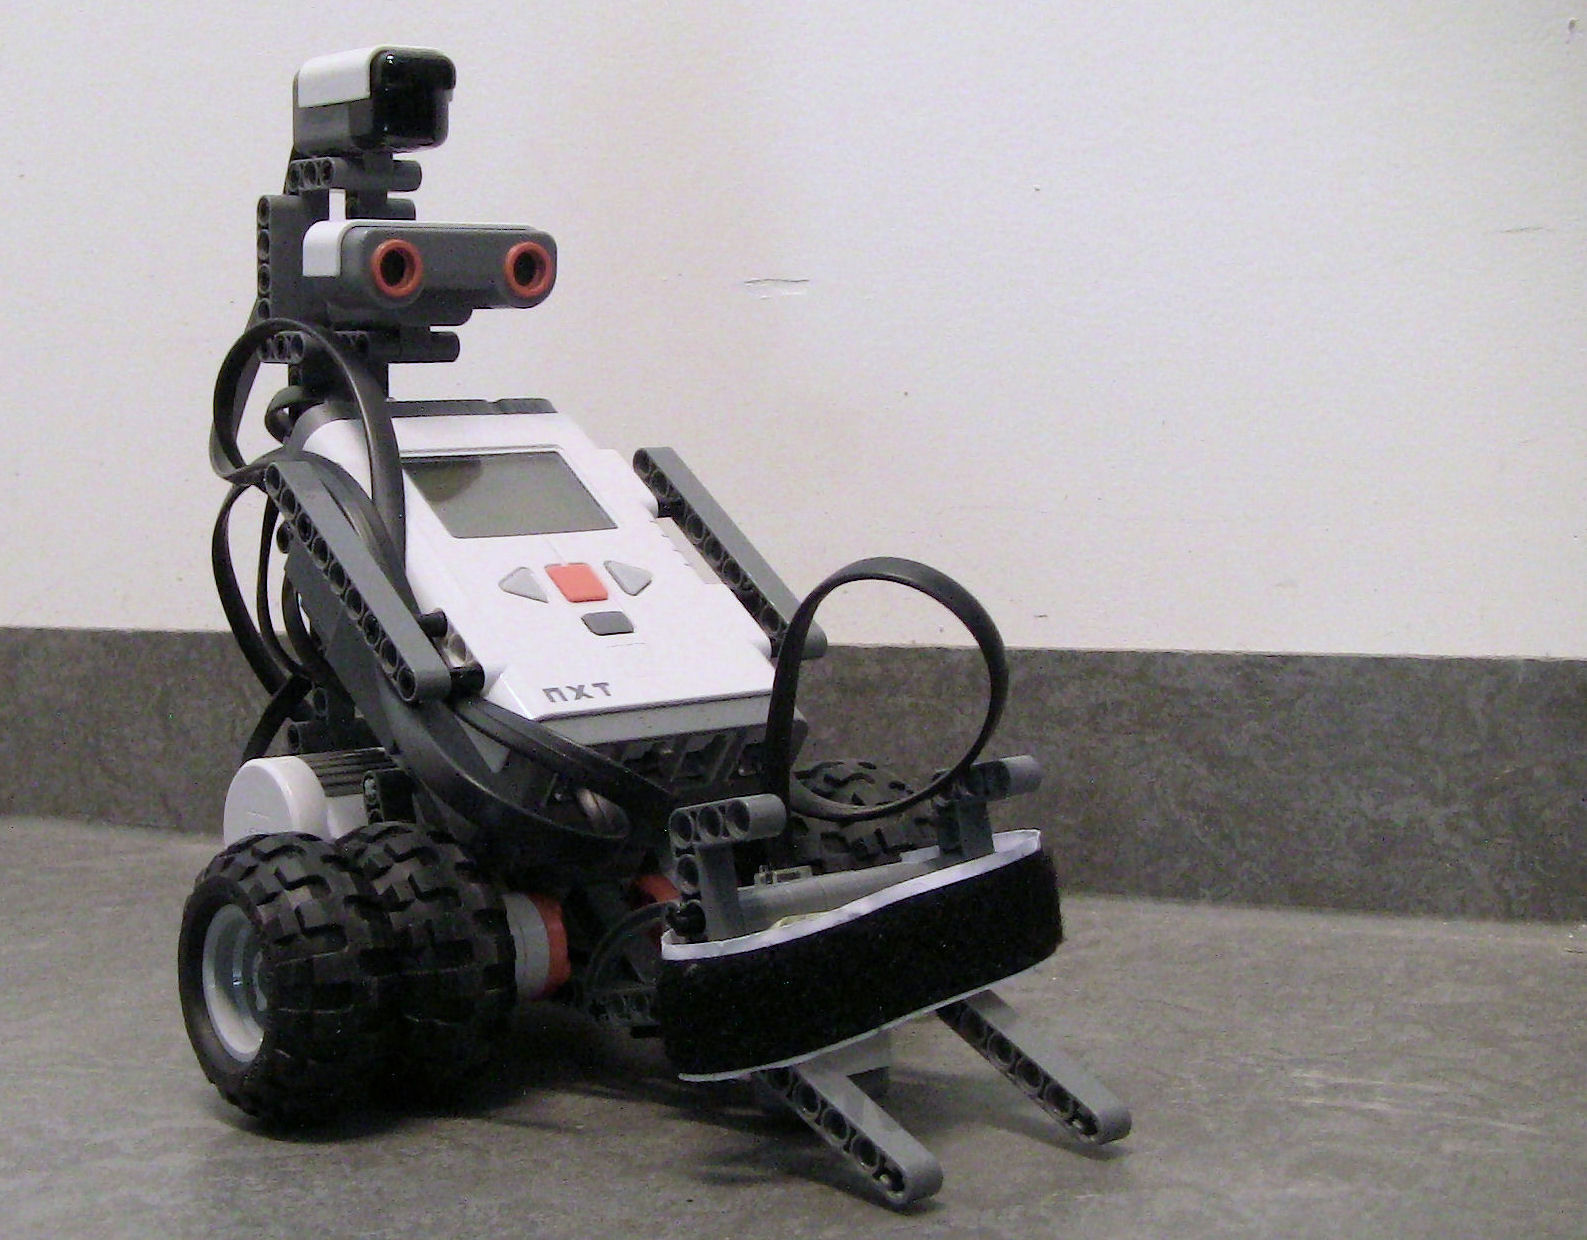
\includegraphics[width=\textwidth]{robotOud3}
		\caption{Schep met klittenband}
		\label{fig:robotOud3}
	\end{subfigure}
\caption{Alternatieve manieren om het voorwerp op te rapen}
\label{fig:robotOud}
\end{figure}

% bouw robot
\begin{figure}
\centering
	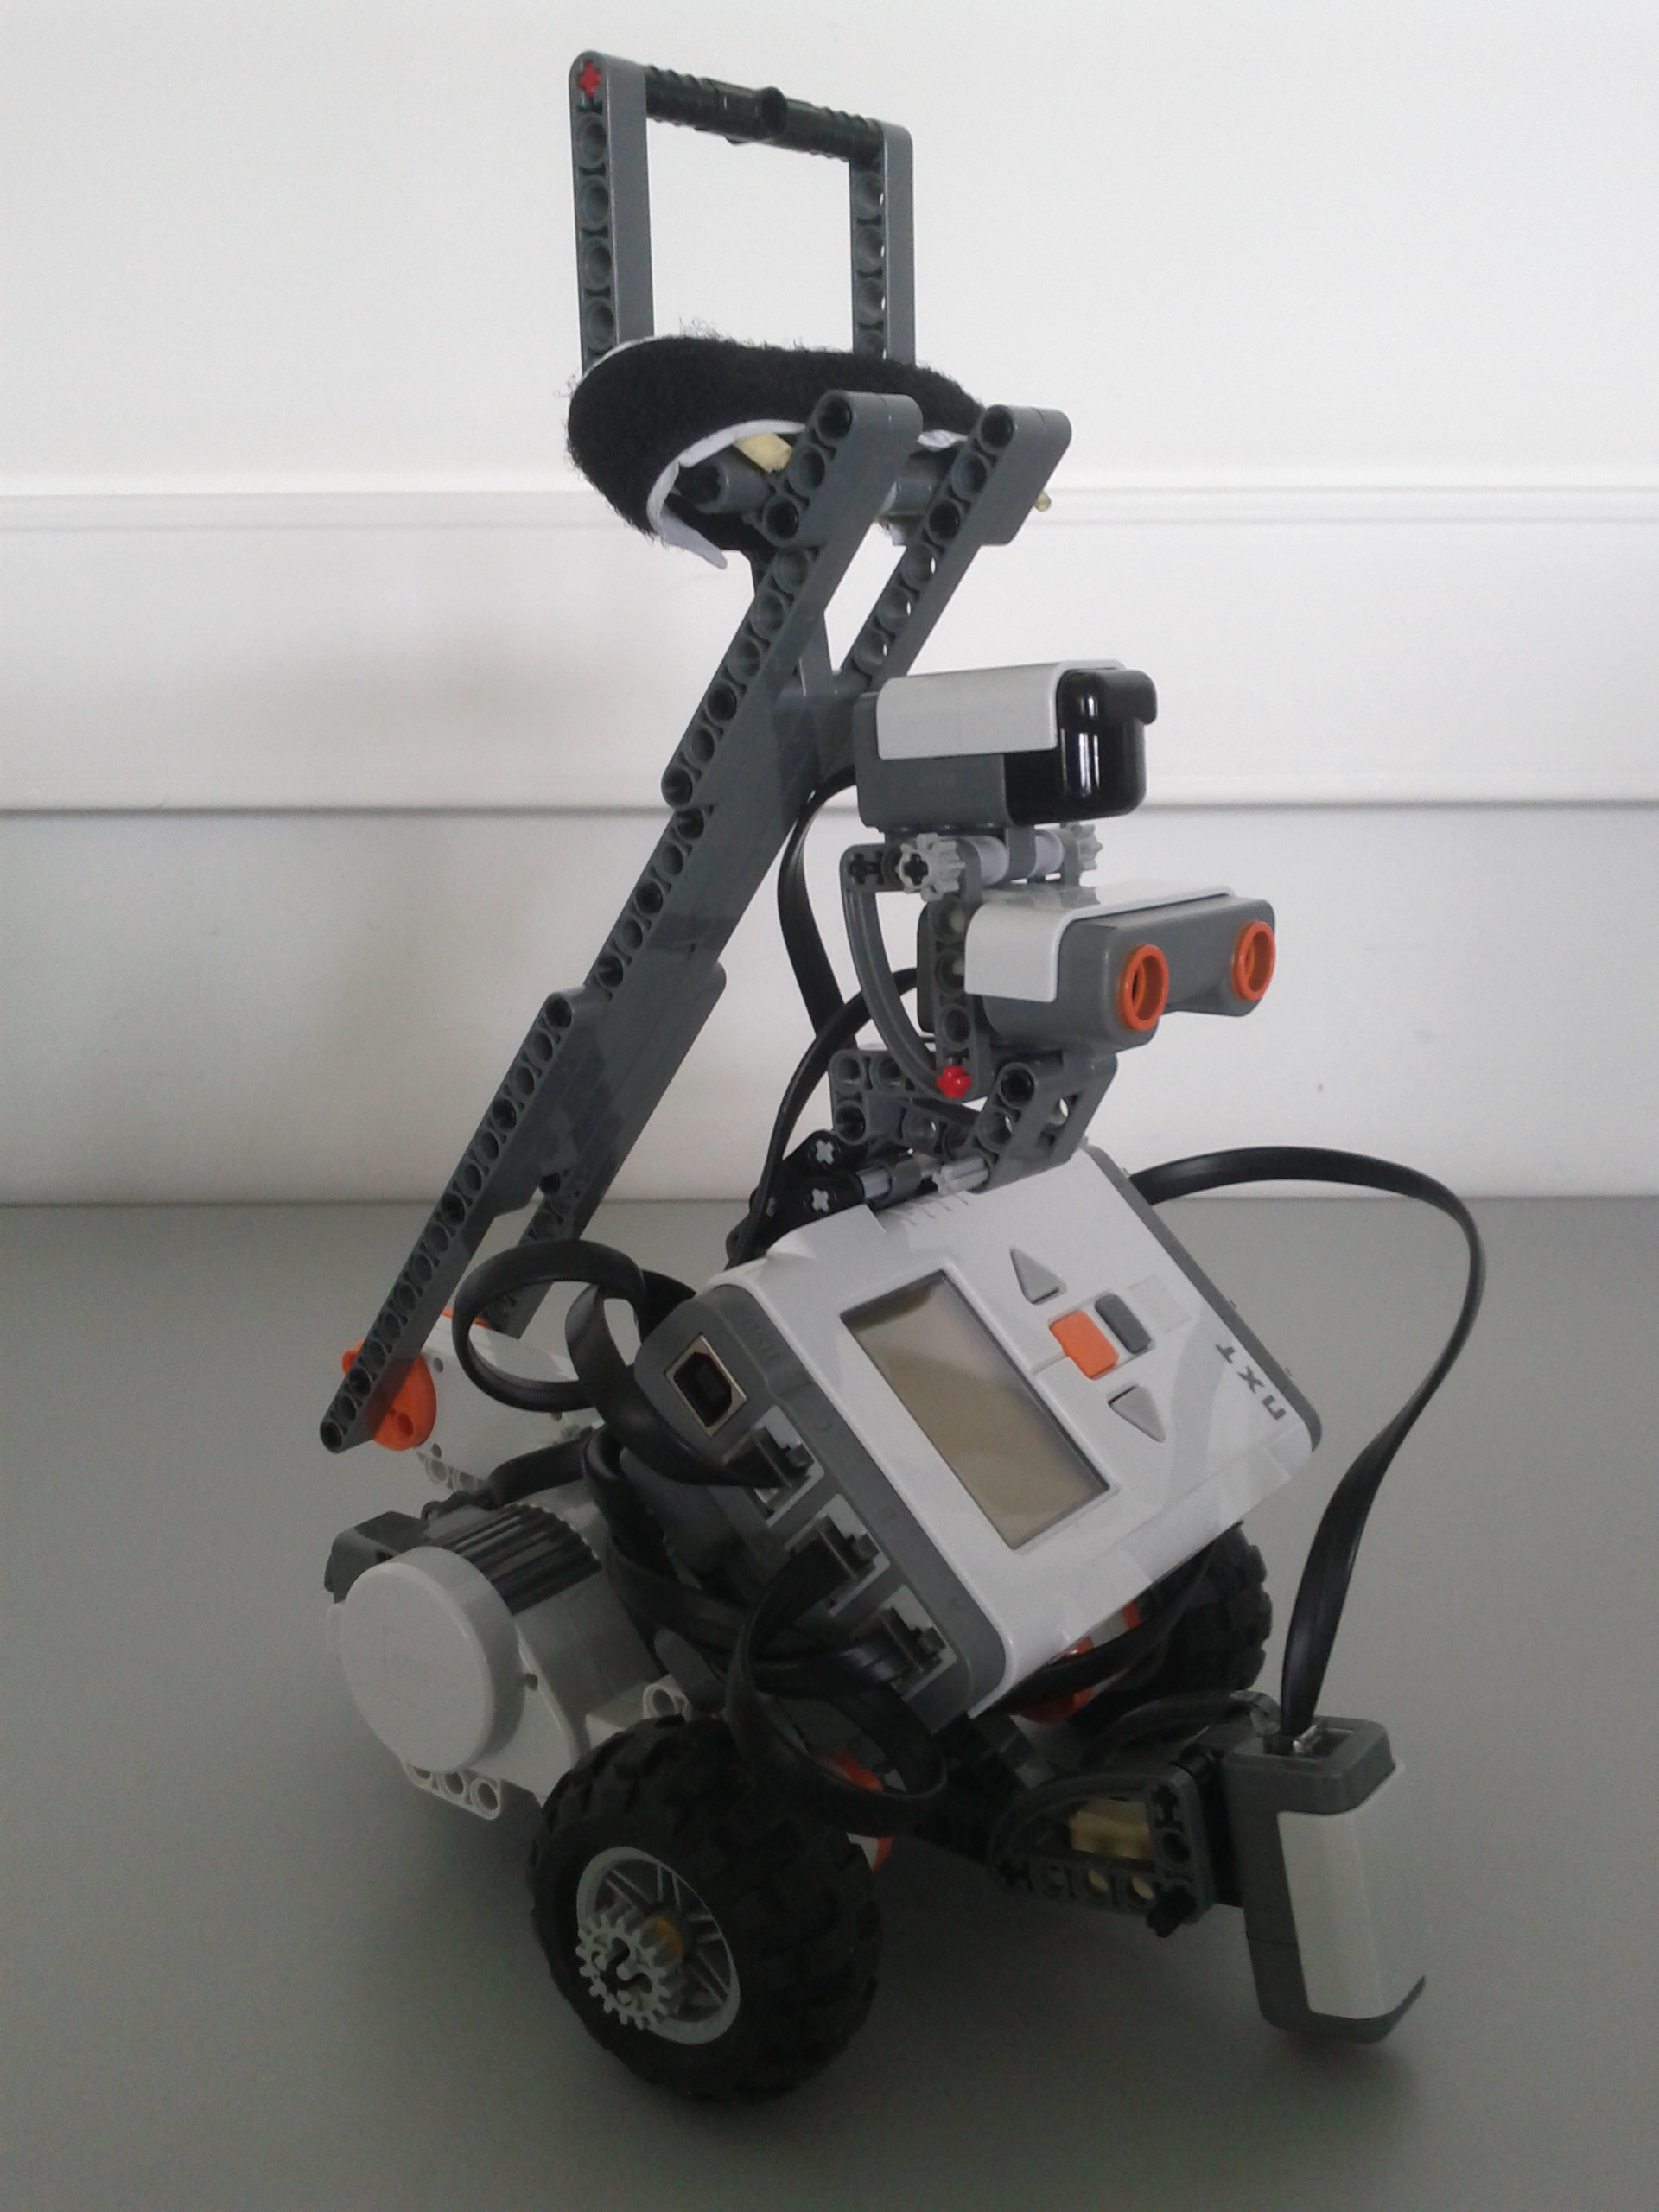
\includegraphics[width=0.5\textwidth]{robotNieuw}
\caption{Huidige ontwerp van de robot}
\label{fig:robotBouw}
\end{figure}

% details robot
\begin{figure}
\centering
	\begin{subfigure}[h]{0.325\textwidth}
	\centering
		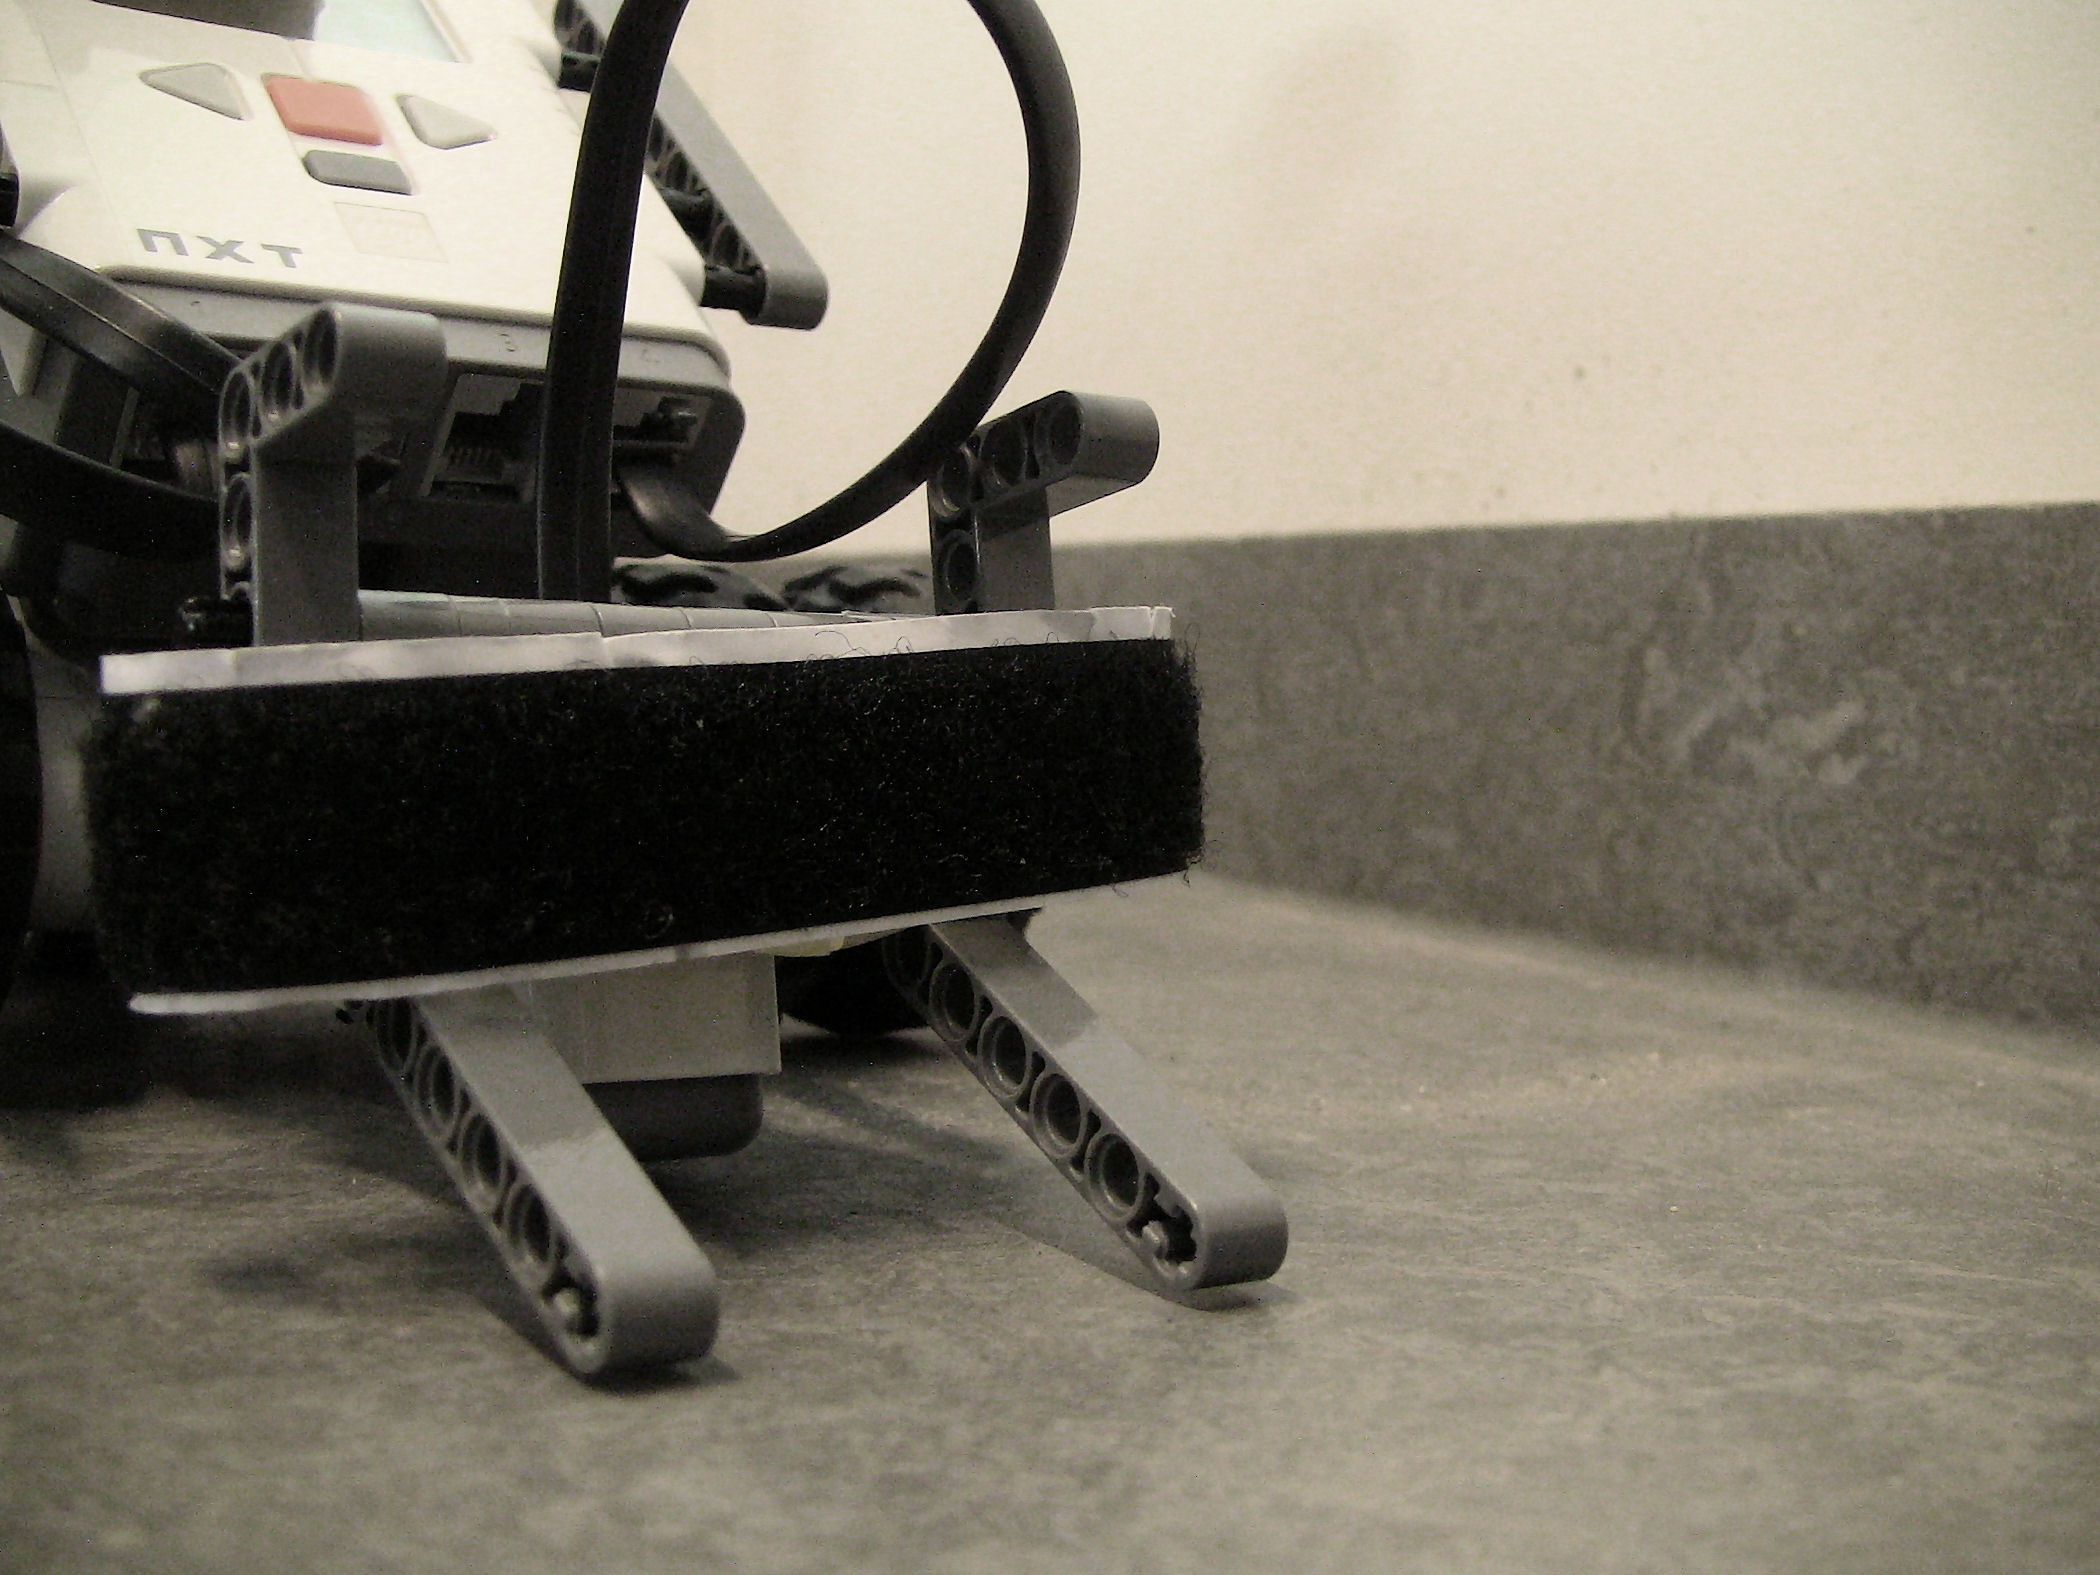
\includegraphics[width=\textwidth]{robotSchep}
		\caption{Lange schep}
	\end{subfigure}
	\begin{subfigure}[h]{0.325\textwidth}
		\centering
		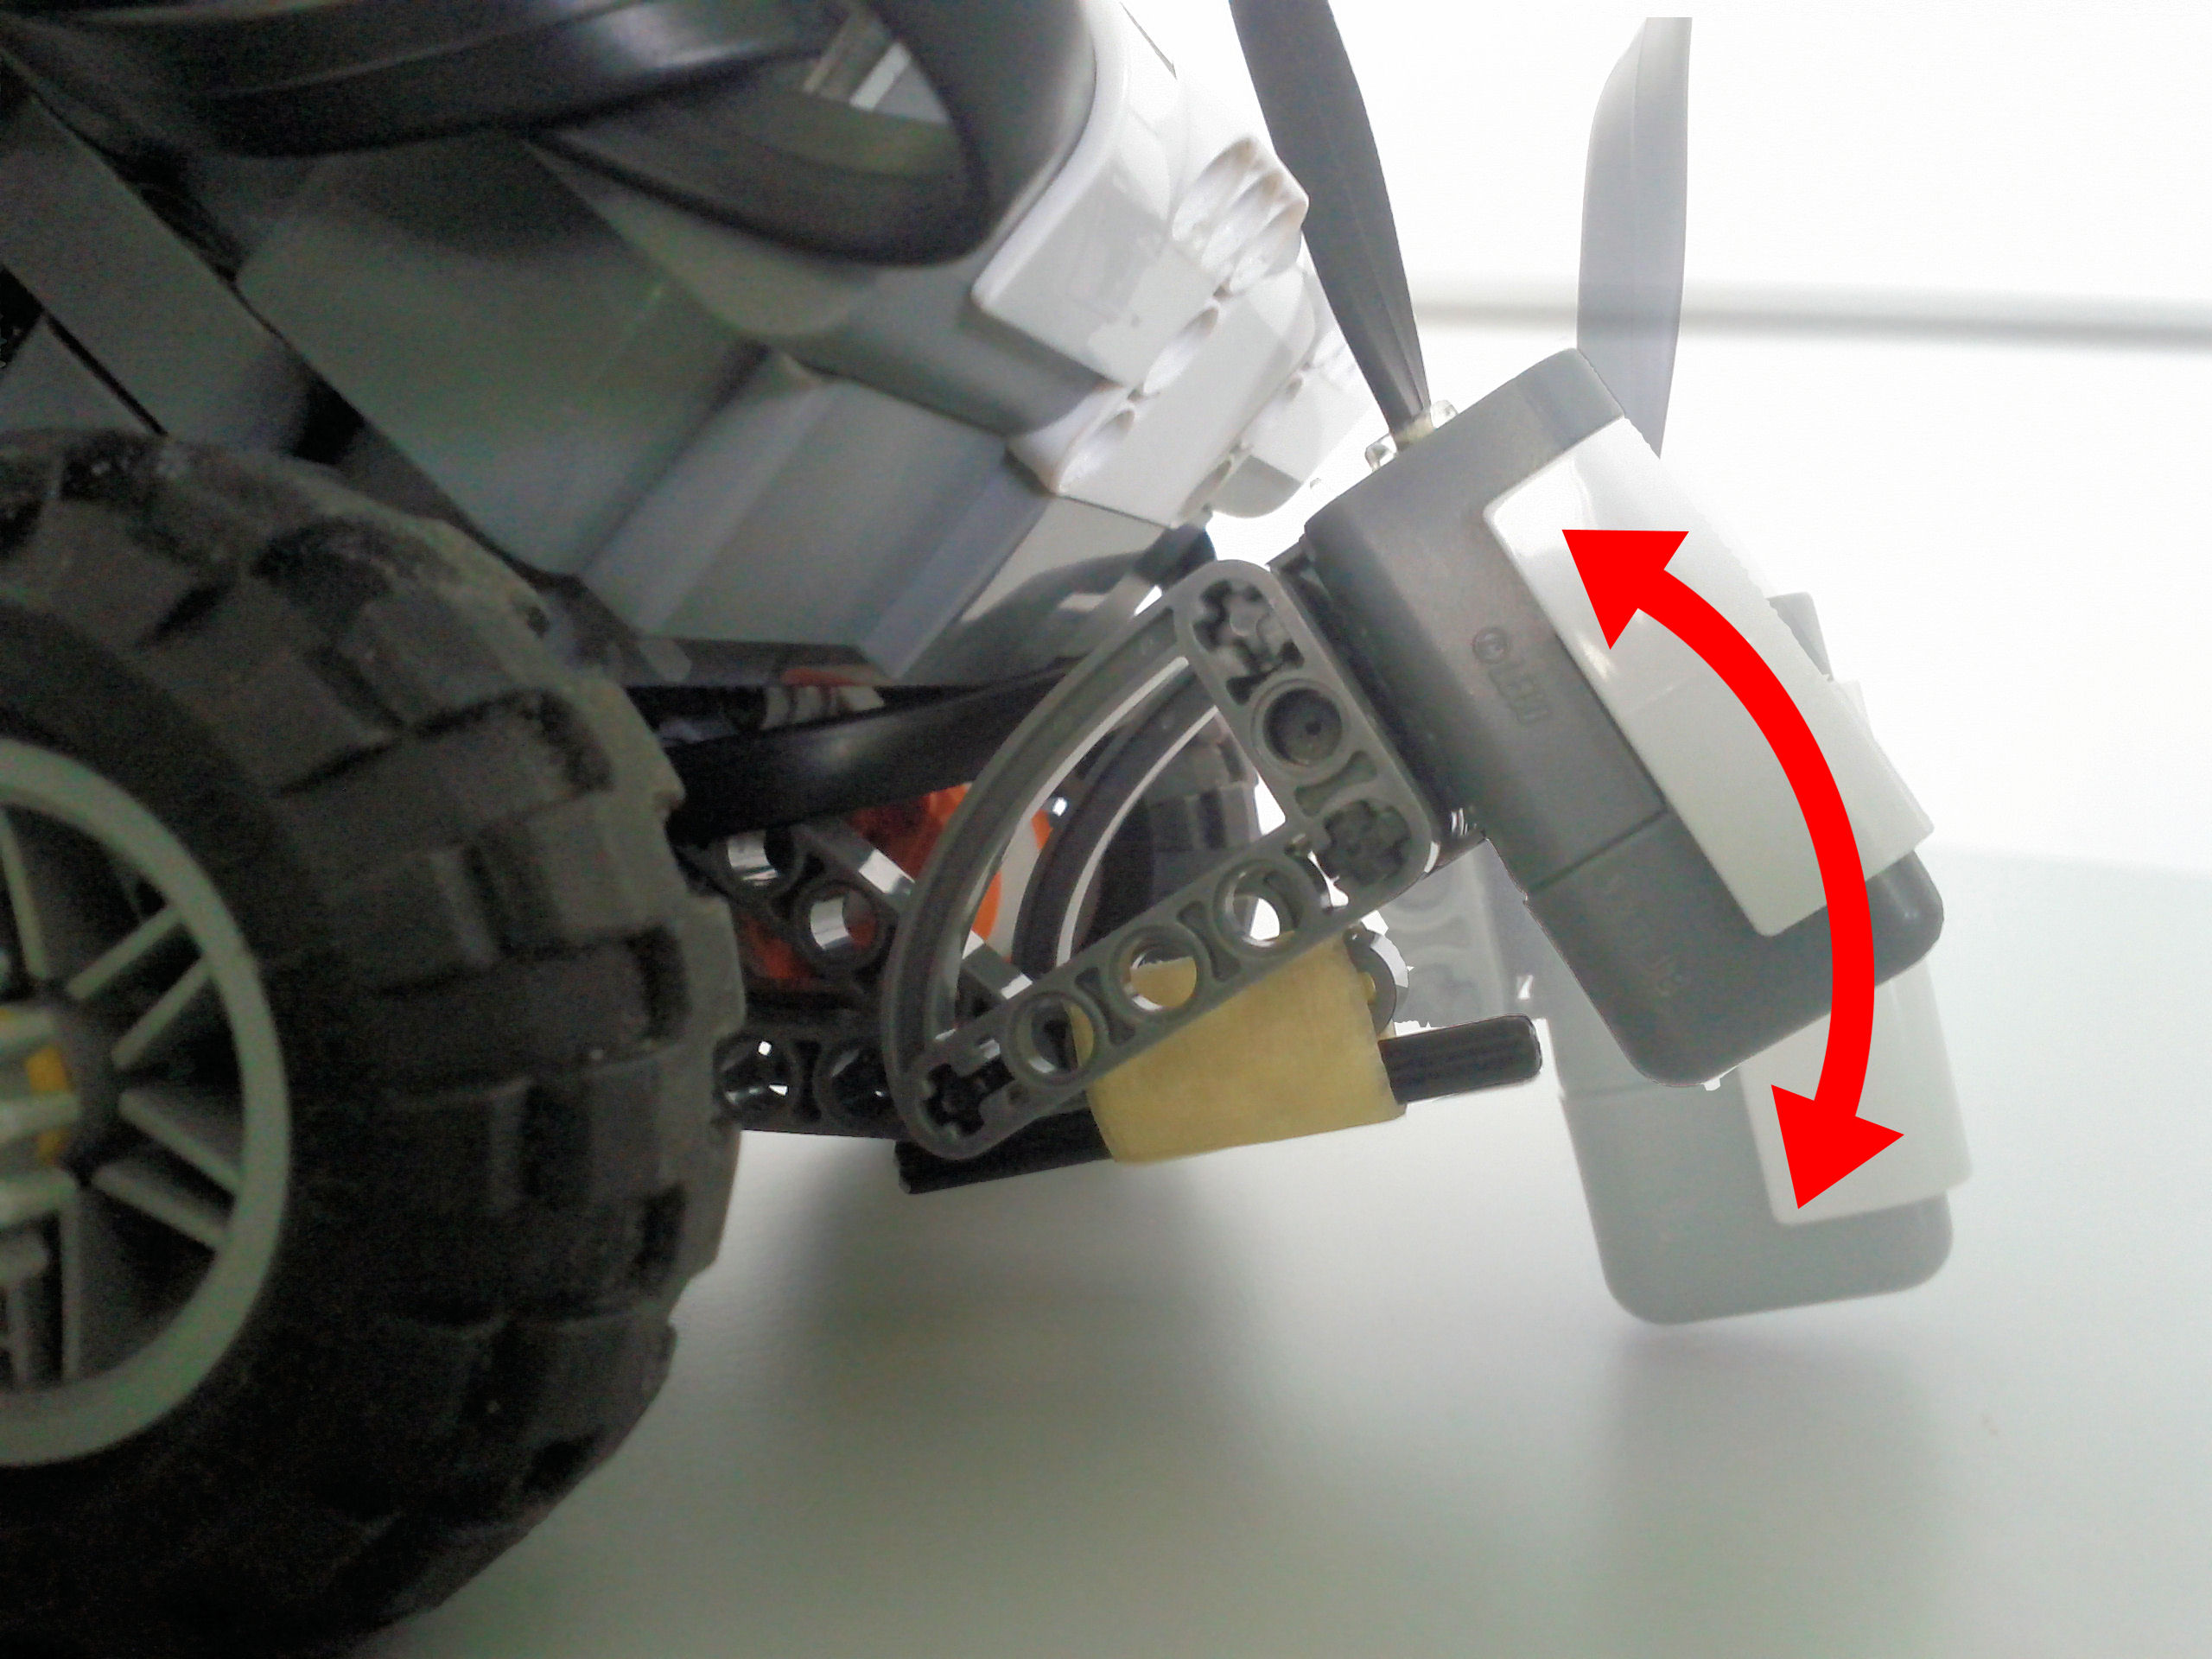
\includegraphics[width=\textwidth]{robotLicht}
		\caption{Lichtsensor op scharnier}
	\end{subfigure}
	\begin{subfigure}[h]{0.325\textwidth}
		\centering
		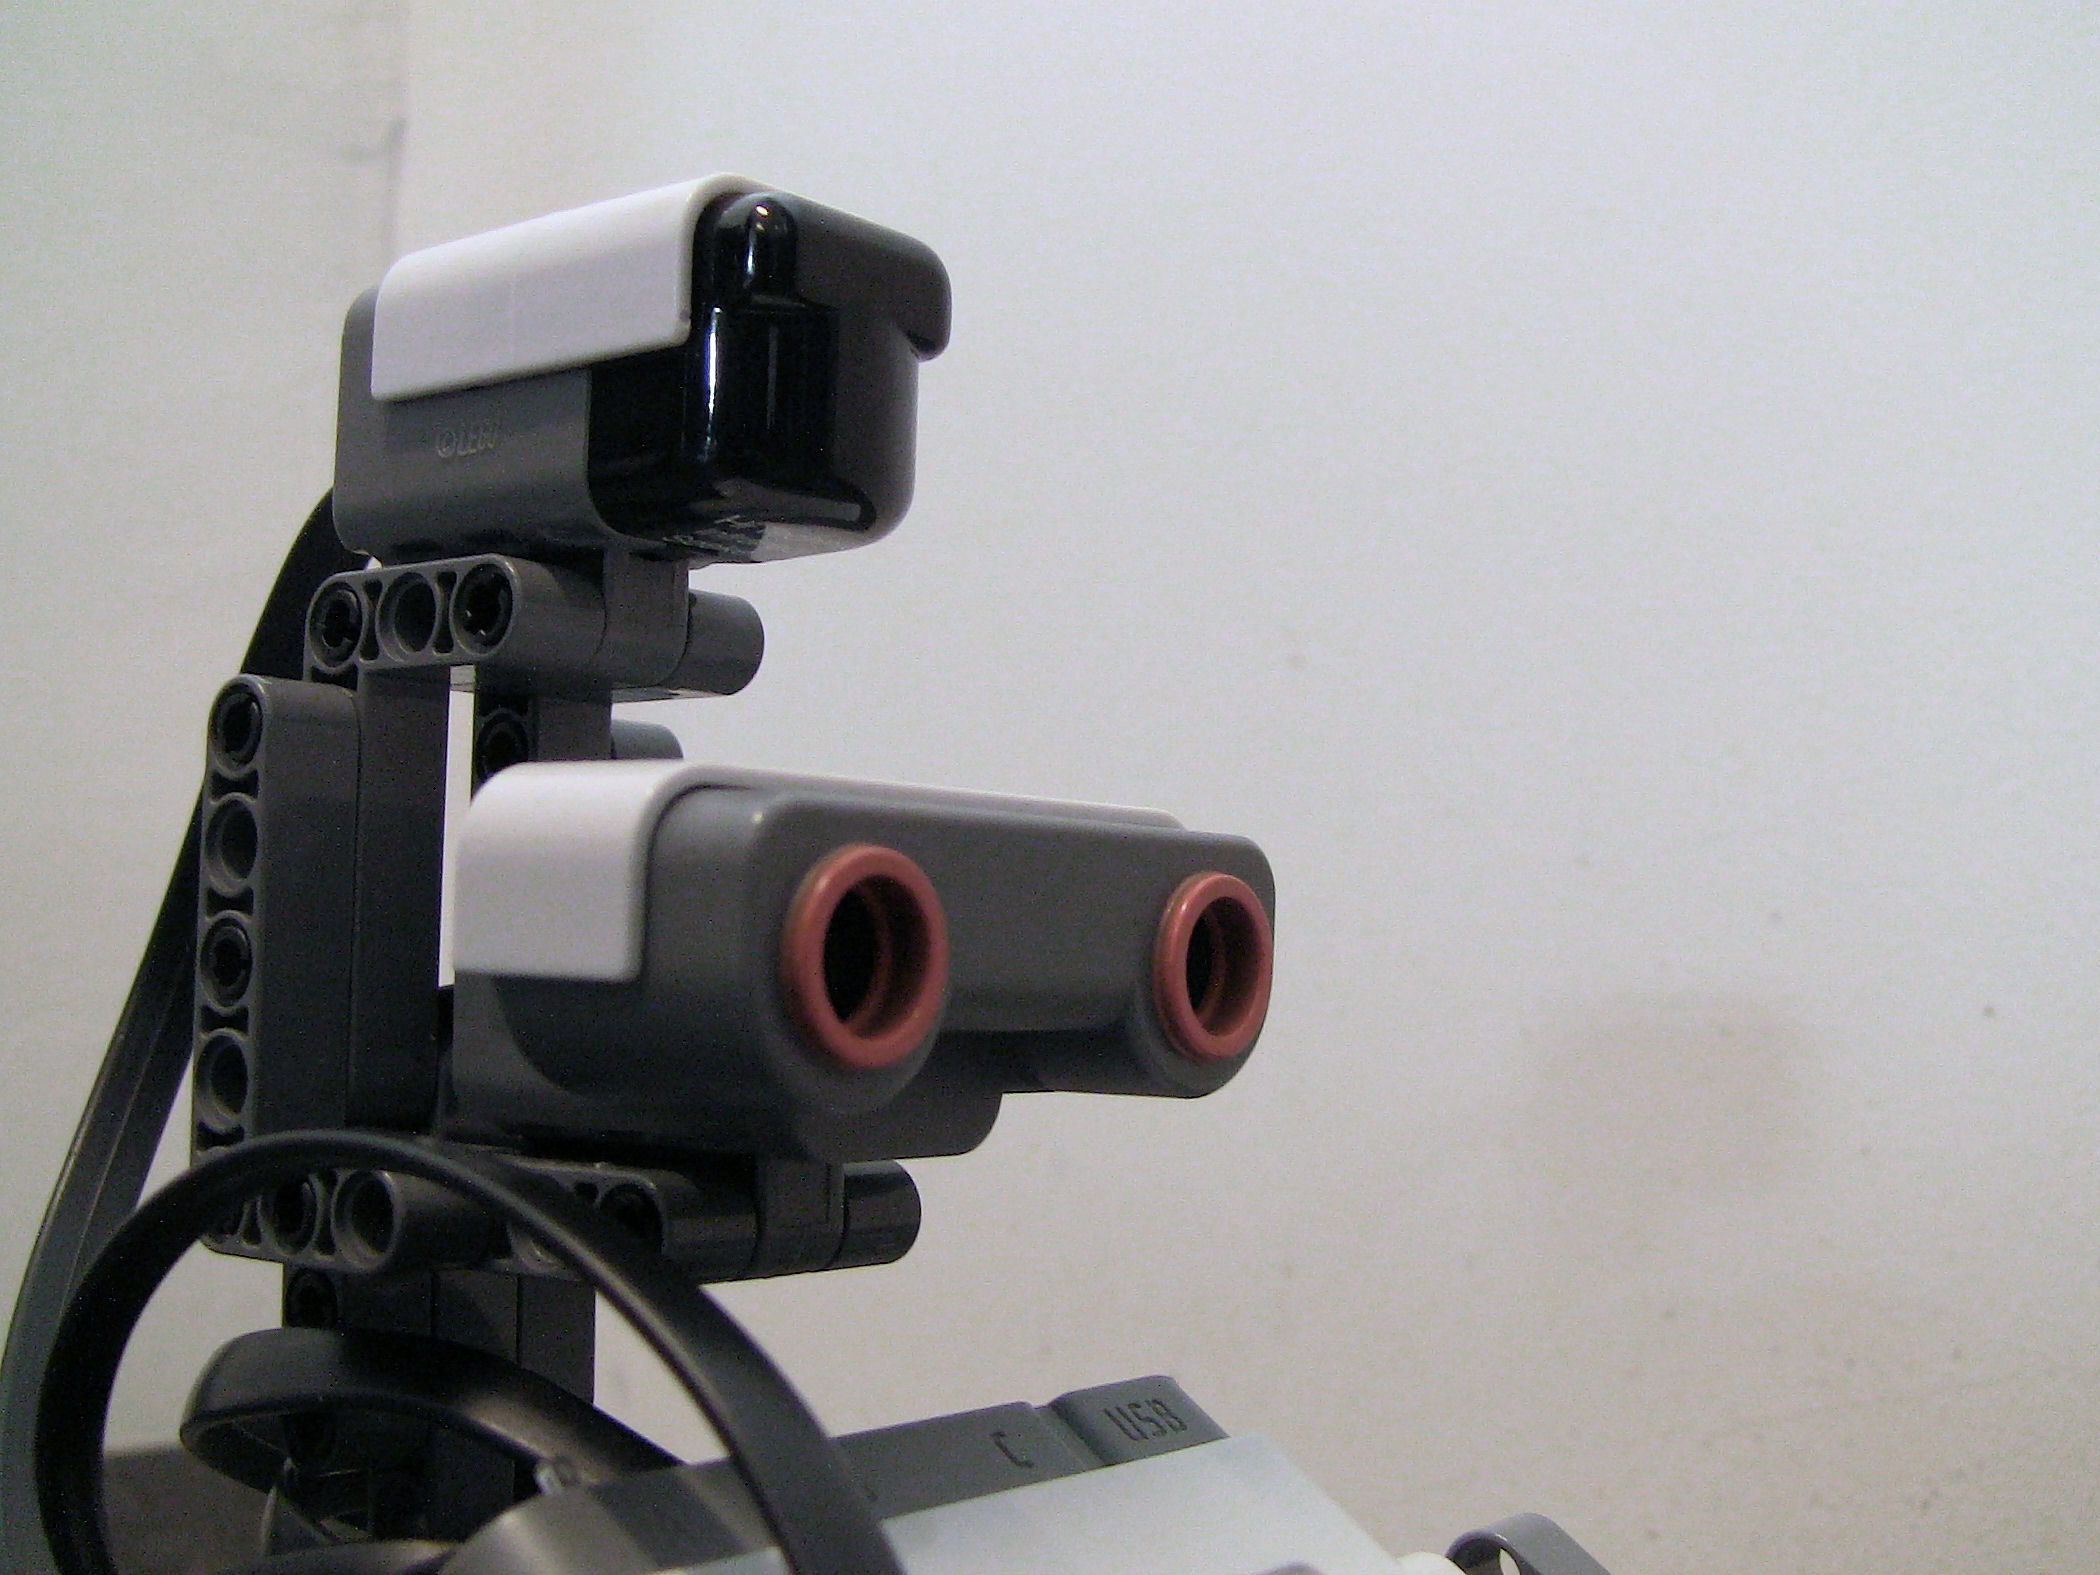
\includegraphics[width=\textwidth]{robotSensoren}
		\caption{Ultrasone- en infraroodsensor}
	\end{subfigure}
\caption{Details van het huidige ontwerp}
\label{fig:robotDetail}
\end{figure}

\subsection{Kalibratie}
\label{ssec:Kalib}
\subsubsection{Motoren}
De robot wordt aangedreven door twee motoren. Beide motoren kunnen onafhankelijk worden aangestuurd. Wanneer de robot rechtdoor rijdt, draaien beide motoren in dezelfde richting. Bij het keren om de as draaien de motoren in tegenovergestelde richtingen. De kalibratie heeft als doel te bepalen hoeveel graden de motoren moeten draaien om de robot respectievelijk \'e\'en cm vooruit de laten rijden en \'e\'en~graad te laten keren.

\subparagraph{E\'en cm vooruit rijden}
Opdat de robot \'e\'en cm vooruit rijdt, moeten de motoren $20,8\degree$ draaien. Het bleek niet nodig deze co\"effici\"ent te wijzigen ten opzichte van het vorige ontwerp. Dit werd getest door de robot dwars op een witte lijn te laten starten en hem $40~cm$ vooruit te laten rijden. De test werd enkele keren herhaald. De robot kwam steeds op de volgende witte lijn uit.

%move forward 20.8 --> perfect

\subparagraph{E\'en graad keren om de as}
De test vertrok van de waarde die gebruikt werd bij het vorige ontwerp:~$2,358\degree$. De robot werd naast een witte lijn neergezet en kreeg een aantal keer de opdracht $90\degree$~rond zijn as te draaien, zowel met een positieve als een negatieve hoek. Door de opdracht een aantal keer te herhalen wordt het gemakkelijker de fout op te merken.
De co\"effici\"ent~$2,330\degree$ gaf het beste resultaat voor positieve en negatieve hoeken.

%eerst 2.358 --> iets te veel
%dan 2.330 --> kleeeeiin iets te weinig
%dan 2.335 --> eerst perfect, toch iets te veel door nieuw achterwiel
%nu 2.330 --> perfect


\subsubsection{Infraroodsensor}
De infraroodsensor neemt een bron van infraroodlicht, zoals een infraroodbal, waar. Hij wordt gebruikt om de stand van de wip te detecteren en bestaat uit vijf onafhankelijke sensoren die elk volgens een andere ori\"entatie gericht staan. De robot maakt enkel gebruik van de middelste sensor omdat de wip zich altijd recht voor de robot zal bevinden. De infraroodsensor geeft een waarde tussen $1$ en $3$, tenzij hij een infraroodbal detecteert. In dat geval geeft hij gemiddeld een waarde rond de~$120$.

\subsubsection{Ultrasone sensor}
De ultrasone sensor zendt ultrasone geluidsgolven uit. Indien een object in de buurt staat, weerkaatsen de golven hierop. De robot ontvangt dan zijn eigen golven opnieuw. De tijd tussen het uitzenden en ontvangen laat toe de afstand tot het object te bepalen.

In een doolhof kan een robot zowel muren als robots tegenkomen. Ook de paaltjes, die de muren omhoog houden, worden gedetecteerd. Om te vermijden dat de paaltjes als muur worden ge\"interpreteerd worden enkel meetwaarden kleiner dan $21$~cm als mogelijke muur beschouwd.

Wanneer de robot in het midden van een tegel staat geeft de sensor een waarde van $16$~cm. Deze waarde wordt gebruikt om de robot te aligneren op basis van de muren (sectie~\ref{sssec:AlgoAllign}).

%US: 16 = muur - om te aligneren op muur,
% treshold = 21 - hieronder is het een muur, geen paalte

\subsubsection{Lichtsensor}
De lichtsensor meet de lichtintensiteit van de omgeving. De sensor kan zelf ook een rood licht uitsturen. Hoe minder licht gereflecteerd wordt door de omgeving, hoe donkerder deze is.

De lichtsensor werd zowel bij goede lichtomstandigheden als bij slechte omstandigheden getest voor alle soorten ondergronden die een doolhof bevat: een paneel, een witte lijn en een zwarte lijn.
De lichtsensor geeft gemiddeld de waarde~$49$ wanneer de robot op het paneel staat, $55$~wanneer hij op een witte lijn staat en $33$~op een zwarte lijn. De robot beschouwt alles boven de $52$ als wit en alles onder $40$ als zwart. Wat hiertussen ligt beschouwt hij als paneel. Door met deze grenzen te werken, wordt een veiligheidsmarge ingebouwd. De kans is klein dat de sensorwaarden verkeerd ge\"interpreteerd worden, ook bij slechte lichtomstandigheden.

%witte lijn lichtsensor: 55
%tegel: 49
%zwart: 33
%--> treshold = 52 (erboven: wit, eronder: paneel)
%				40 (eronder: zwart, erboven: paneel)

\newpage

% == ALGORITMES == %
\section{Algoritmes}
\label{sec:Algo}

Om het spel te spelen dient de robot de doolhof zo nauwkeurig mogelijk te verkennen (sectie~\ref{ssec:AlgoVerken}). Hierbij moet hij rekening houden met onnauwkeurigheden in zijn besturing (sectie~\ref{sssec:AlgoAllign}) en met de verschillende onderdelen die een doolhof bevat: barcodes (sectie~\ref{sssec:AlgoBar}), wippen (sectie~\ref{sssec:AlgoWip}) en voorwerpen (sectie~\ref{sssec:AlgoZoek}). Bovendien dienen andere robots gedetecteerd te worden zodat botsingen vermeden worden (sectie~\ref{sssec:AlgoCollision}).

De robot dient ook samen te werken met zijn teamgenoot (sectie~\ref{ssec:AlgoSamen}). Hierbij moet hij gebruik kunnen maken van de informatie die deze stuurt (sectie~\ref{sssec:AlgoMappen}) en moet hij een manier vinden om de teamgenoot te bereiken (sectie~\ref{sssec:AlgoTeam}).


% == Verkennen == %
\subsection{Doolhoven verkennen}
\label{ssec:AlgoVerken}

% = aligneren = %
\subsubsection{Positie en ori"entatie corrigeren}
\label{sssec:AlgoAllign}
Het is niet mogelijk om de robot 100\% nauwkeurig te laten rijden: de motoren kunnen immers slechts tot op een bepaalde nauwkeurigheid ingesteld worden. Om de besturing toch betrouwbaar te maken is het nodig de robot zichzelf te laten aligneren. Dit gebeurt bij elke tegel.
De methode bestaat uit twee basisalgoritmes: op basis van een witte lijn en op basis van een muur.

\subparagraph{Aligneren op basis van een witte lijn}
De robot rijdt vooruit tot de lichtsensor wit detecteert (figuur~\ref{fig:AlgoWit1} en~\ref{fig:AlgoWit2}). Hij rijdt verder tot de sensor weer paneel detecteert (figuur~\ref{fig:AlgoWit3}). Pas na een tweede positieve check van de sensor stopt de robot. Zo wordt vermeden dat de robot stopt op de scheiding van twee panelen. De robot staat nu net over de witte lijn. De robot rijdt verder vooruit tot de wielas net boven de witte lijn staat (figuur~\ref{fig:AlgoWit4}). Vervolgens draait de robot om zijn as tot de lichtsensor weer wit detecteert (figuur~\ref{fig:AlgoWit5}). De robot aligneert op basis van de muur (figuur~\ref{fig:AlgoWit6}) en draait~90\degree~in de andere richting (figuur~\ref{fig:AlgoWit7}). Hij rijdt tenslotte nog $20$~cm voorwaarts. De robot staat nu evenwijdig aan de muren en in het midden van de tegel.

\begin{figure}[h]
\centering
	\begin{subfigure}[h]{0.24\textwidth}
		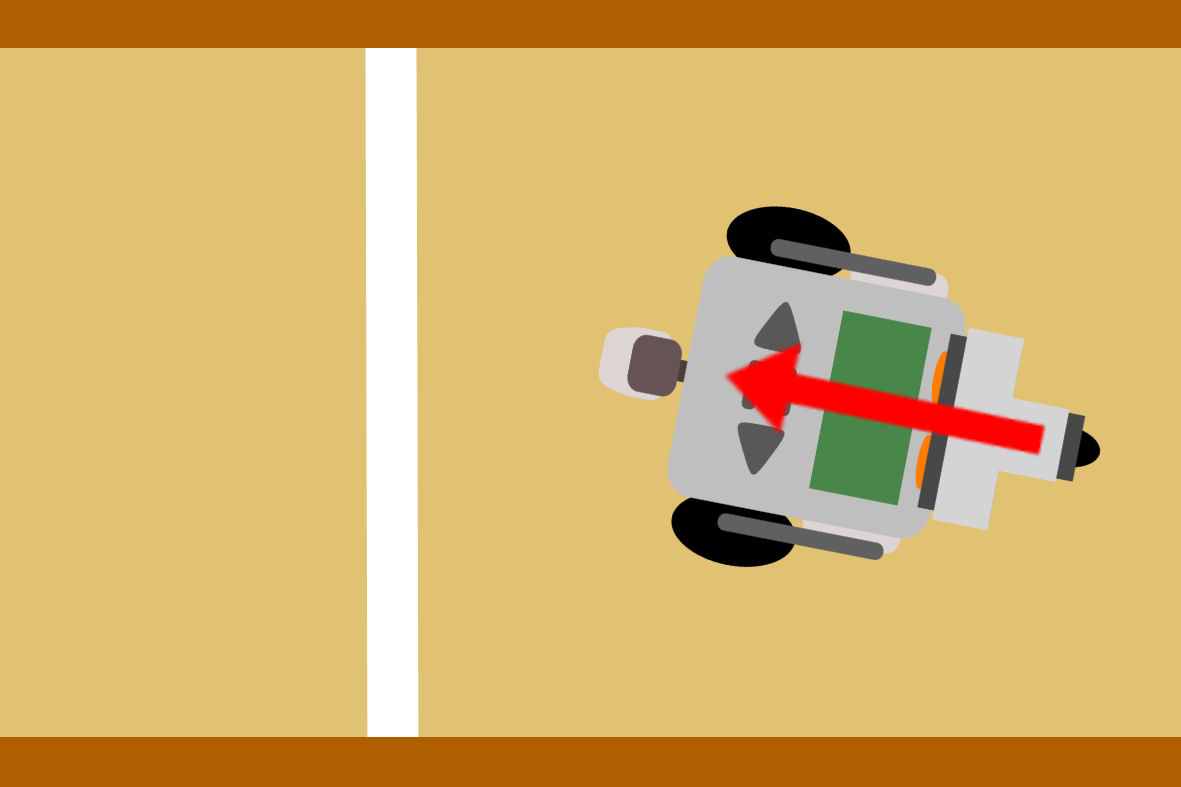
\includegraphics[width=\textwidth]{WitteLijn1}
		\caption{ }
		\label{fig:AlgoWit1}
	\end{subfigure}
	\begin{subfigure}[h]{0.24\textwidth}
		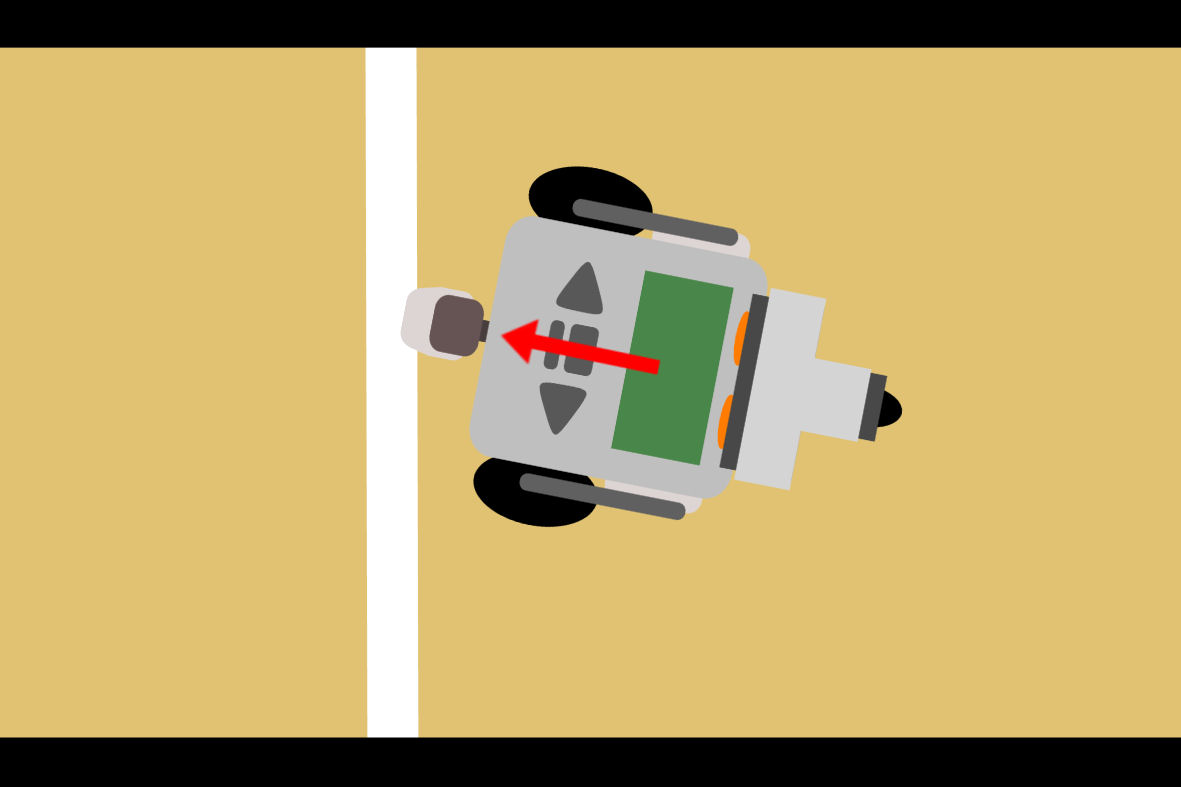
\includegraphics[width=\textwidth]{WitteLijn2}
		\caption{ }
		\label{fig:AlgoWit2}
	\end{subfigure}
	\begin{subfigure}[h]{0.24\textwidth}
		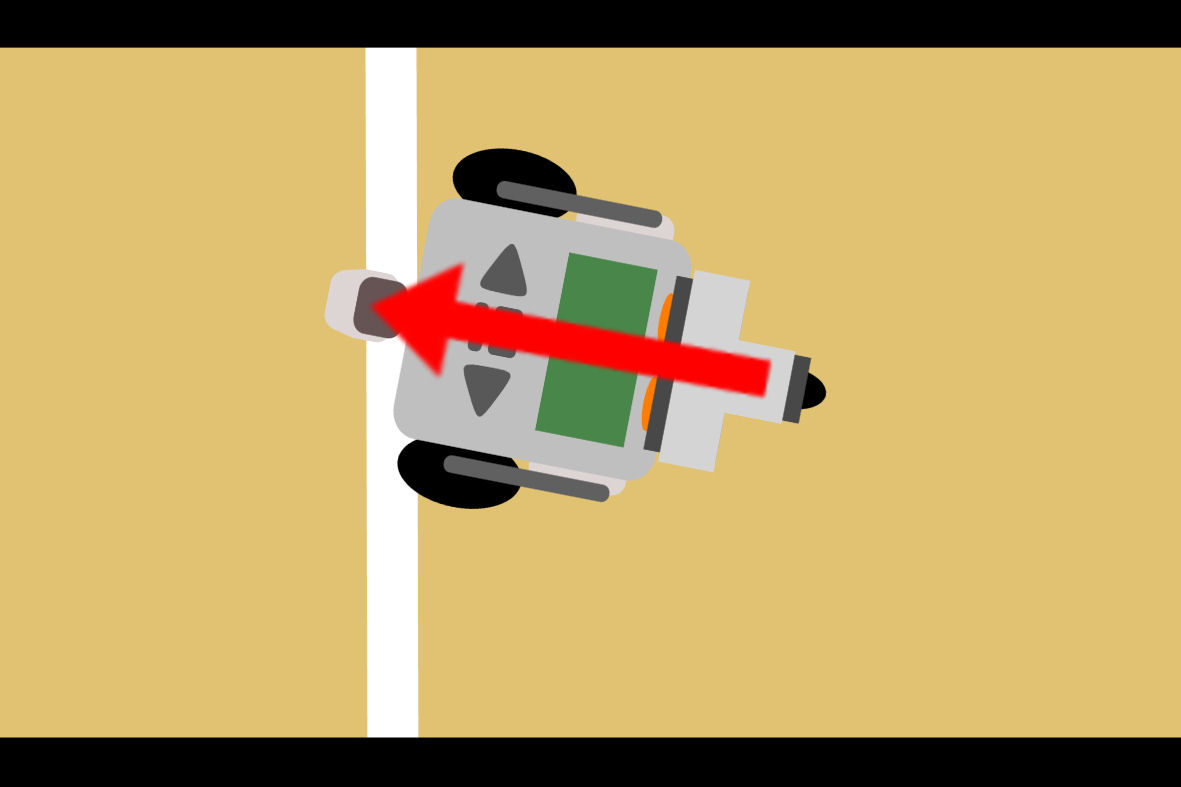
\includegraphics[width=\textwidth]{WitteLijn3}
		\caption{ }
		\label{fig:AlgoWit3}
	\end{subfigure}
	\begin{subfigure}[h]{0.24\textwidth}
		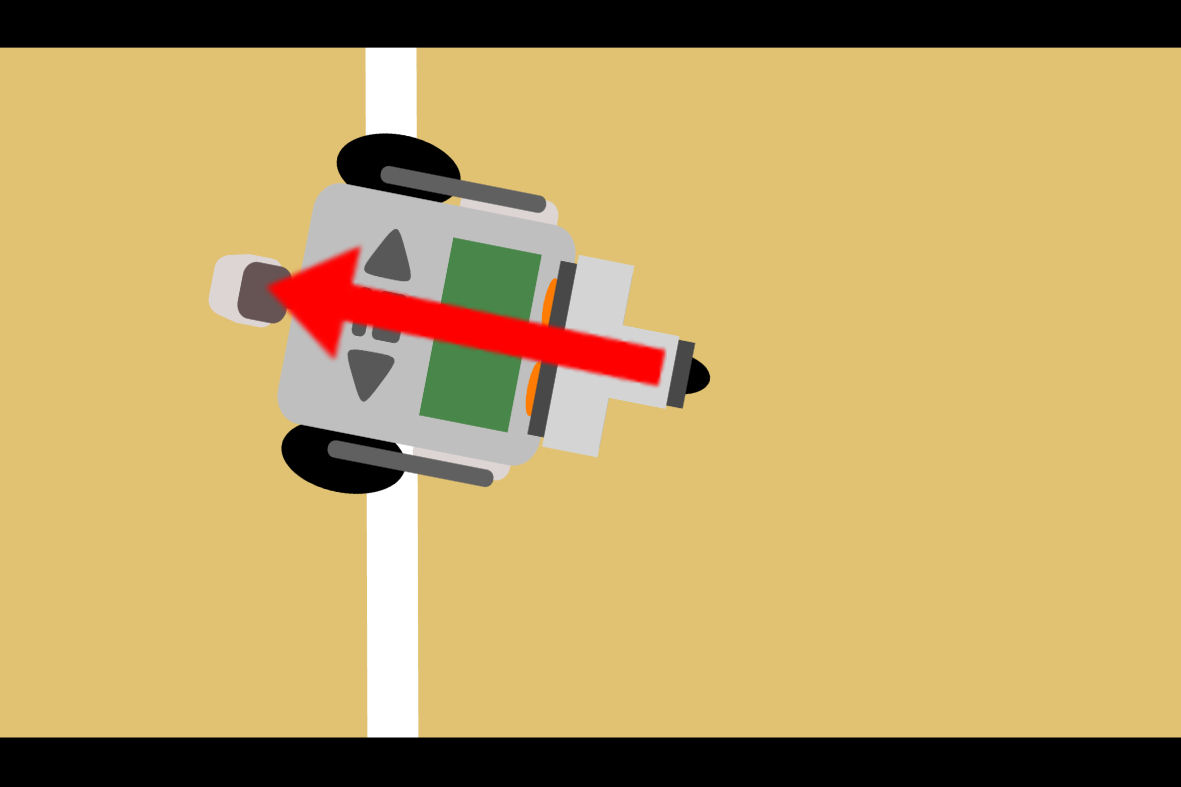
\includegraphics[width=\textwidth]{WitteLijn4}
		\caption{ }
		\label{fig:AlgoWit4}
	\end{subfigure}\\ \vspace{0.2cm}
	\begin{subfigure}[h]{0.24\textwidth}
		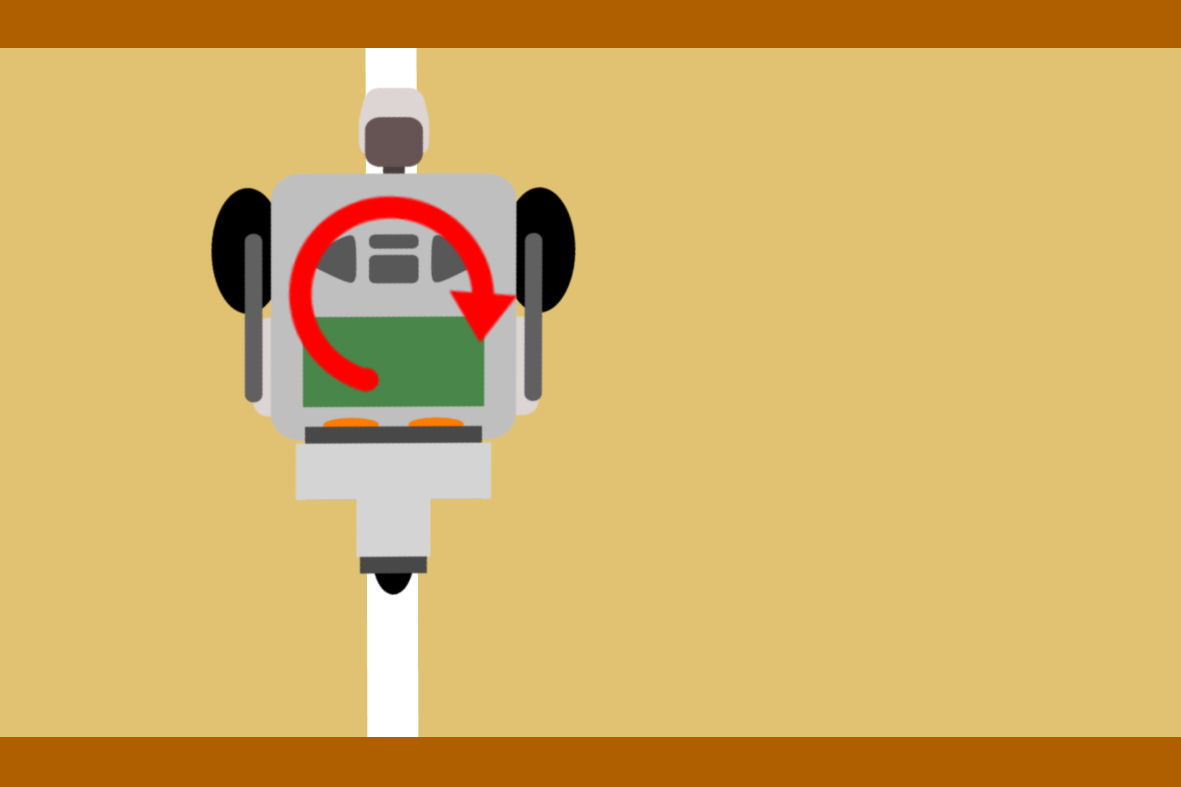
\includegraphics[width=\textwidth]{WitteLijn5}
		\caption{ }
		\label{fig:AlgoWit5}
	\end{subfigure}
	\begin{subfigure}[h]{0.24\textwidth}
		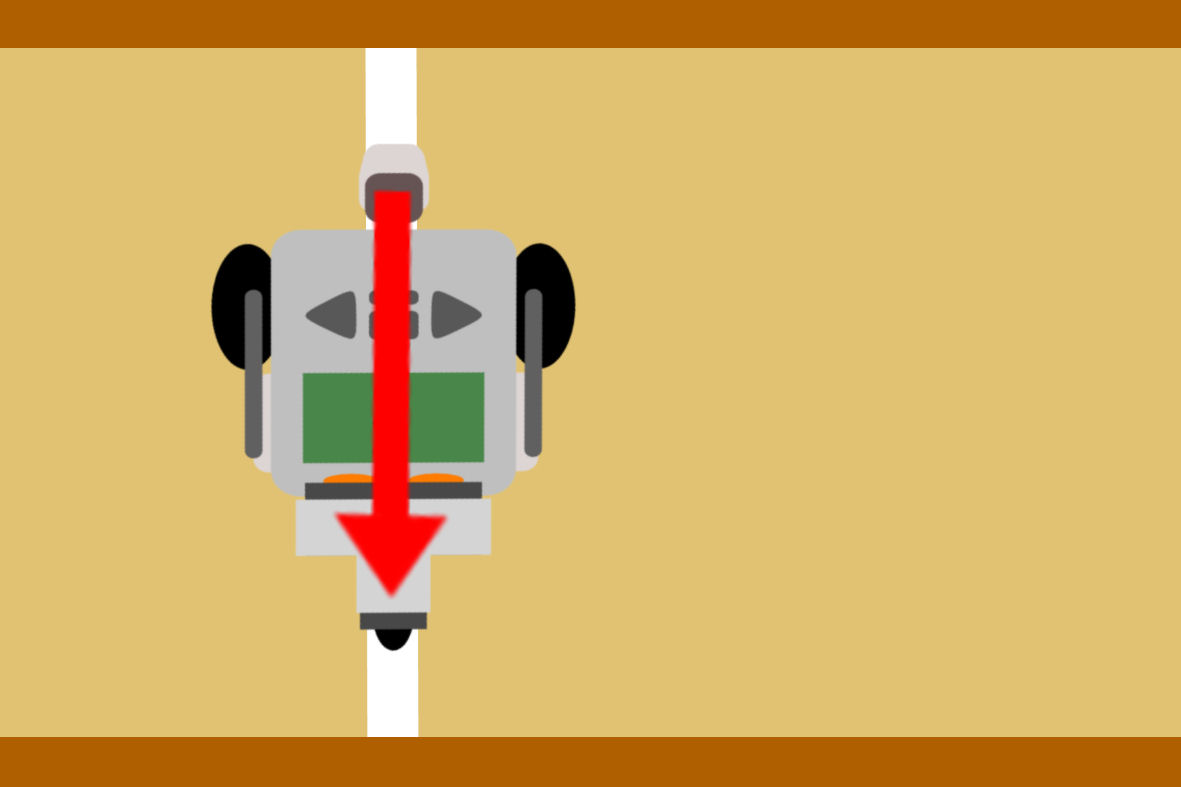
\includegraphics[width=\textwidth]{WitteLijn6}
		\caption{ }
		\label{fig:AlgoWit6}
	\end{subfigure}
	\begin{subfigure}[h]{0.24\textwidth}
		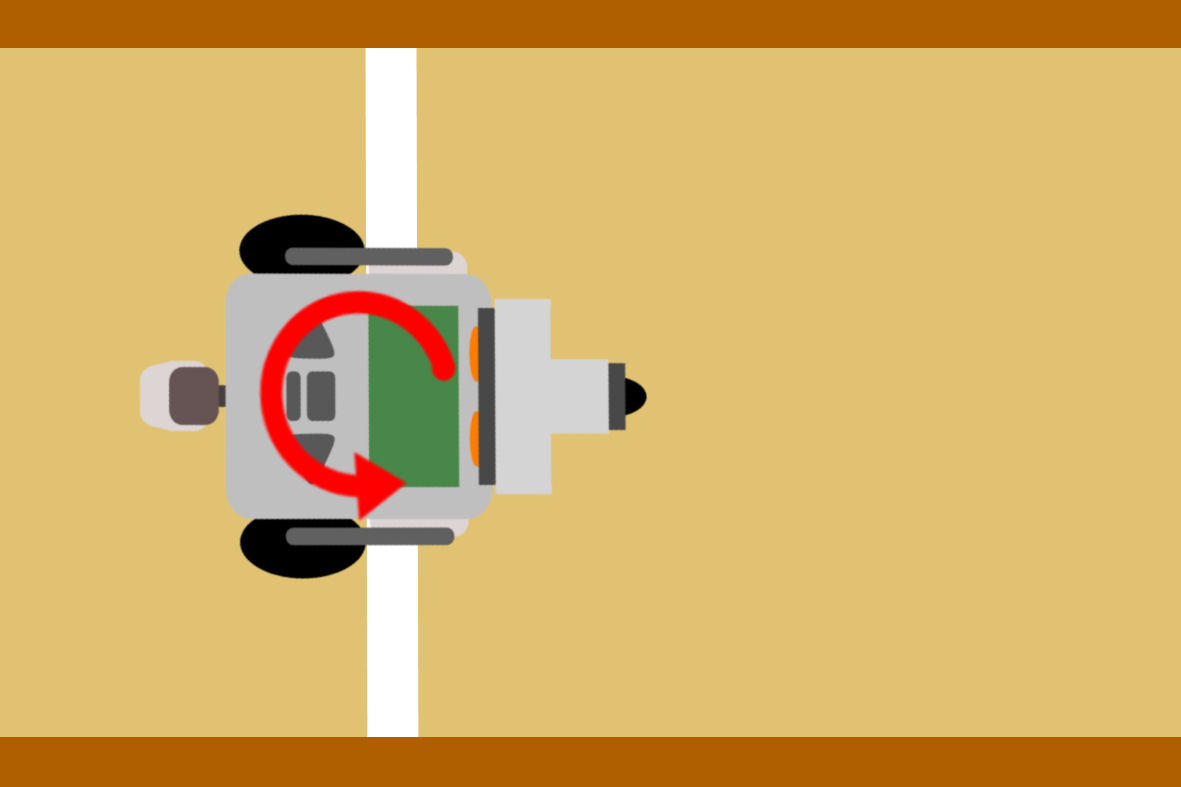
\includegraphics[width=\textwidth]{WitteLijn7}
		\caption{ }
		\label{fig:AlgoWit7}
	\end{subfigure}\\
	\caption{Algoritme om de positie en ori"entatie van de robot te corrigeren}
	\label{fig:AlgoWit}
\end{figure}

\subparagraph{Aligneren op basis van muren}
Dit algoritme wordt enkel uitgevoerd wanneer de robot lateraal op een witte lijn staat. Indien de ultrasone sensor een te hoge waarde geeft, besluit de robot dat er geen muur voor hem staat en corrigeert hij zichzelf niet. Indien er wel een muur is, rijdt de robot naar voren of naar achteren tot de ultrasone sensor een waarde van $16$ geeft. De robot staat dan in het midden van de witte lijn.

% = barcodes = %
\subsubsection{Barcode}
\label{sssec:AlgoBar}
Een barcode bestaat uit acht stroken van $2$~cm, waarvan de eerste en de laatste strook steeds zwart zijn. De andere stroken kunnen zwart of wit zijn en vormen samen de waarde van de barcode. De robot kijkt tijdens het rijden steeds of de lichtsensor een zwarte ondergrond detecteert. Indien dit het geval is, rijdt de robot $17$~cm vooruit zodat hij achter de barcode eindigt. Ondertussen leest hij elke $2$~cm de waarde van de lichtsensor af. De combinatie van deze waarden geeft de waarde van de barcode.\\

% methode om te meten hoeveel je hebt gereden: tacho

Wanneer de gevonden barcode een voorwerp aanduidt, weet de robot dat de volgende tegel een `dead-end' is zonder deze te moeten bezoeken. Deze tegel wordt automatisch toegevoegd aan de map en ingesteld als `verkend'. Indien dit het gezochte voorwerp is, raapt de robot dit op.
Analoog voor een barcode die een wip aanduidt: de volgende drie tegels, waarvan er twee een wip bevatten, worden automatisch toegevoegd aan de map.


% = wip = %
\subsubsection{Wip}
\label{sssec:AlgoWip}
Een wip bestaat uit vier tegels die kantelen wanneer een robot erover rijdt. Slechts twee tegels zijn bereikbaar. Het is enkel mogelijk een wip op te rijden langs de zijde die naar beneden staat.

Een wip wordt voorafgegaan door barcodes die de wip identificeren. Onder een wip ligt een infraroodbal. Wanneer de robot infraroodlicht detecteert, weet hij dat hij voor een wip staat, maar deze niet kan oversteken. \\

De robot rijdt vaak onnauwkeurig bij het nemen van de wip. Hij zal een wip daarom zoveel mogelijk vermijden. Slechts wanneer de onverkende tegels enkel bereikbaar zijn via een wip, rijdt de robot naar de dichtstbijzijnde wip die toegang geeft tot die tegels.

Wanneer deze wip open is, zal de robot hem oversteken. Wanneer de wip gesloten is, kan de robot de wip openen met behulp van zijn schep. Deze functie kan ook worden uitgeschakeld. In dat geval zal de robot naar een andere wip rijden of blijven tot een andere robot de wip opent.

% = wip openen = %
\subparagraph{Een wip openen} 
Dit algoritme wordt uitgevoerd wanneer de robot voor een gesloten wip staat. De robot rijdt achterwaarts en aligneert zich op de witte lijn voor de barcode. Na het aligneren staat de robot midden op de tegel met barcode. De robot draait~$180\degree$ om zijn as en laat zijn schep $75\degree$~dalen zodat deze op de wip ligt. Dit wordt getoond in figuur~\ref{fig:robotWip}. Vervolgens daalt de schep nog~$35\degree$ terwijl de robot $20$~cm vooruit rijdt. Zo trekt hij de wip open. De schep beweegt weer omhoog terwijl de robot nog eens $20$~cm vooruit rijdt. De robot draait $180\degree$ om zijn as en controleert of de wip echt geopend werd. Als dit het geval blijkt te zijn, kan hij de wip oversteken.

De robot dient volgens het protocol twee keer een `lock' aan te vragen tijdens deze operatie, de wip kantelt immers tweemaal. 
Door een tegel te `locken' weten de andere robots dat de robot zich naar die tegel zal bewegen. Zij zullen deze tegel vermijden tot hij terug vrij komt. Door bij te houden wanneer een wip `gelocked' wordt, kan een robot bepalen wat de stand van de wip is zonder deze te zien. Dit algoritme wordt echter niet ge\"implementeerd, maar mogelijk maken andere teams gebruik van de optie.

\begin{figure}[hb!]
	\centering
	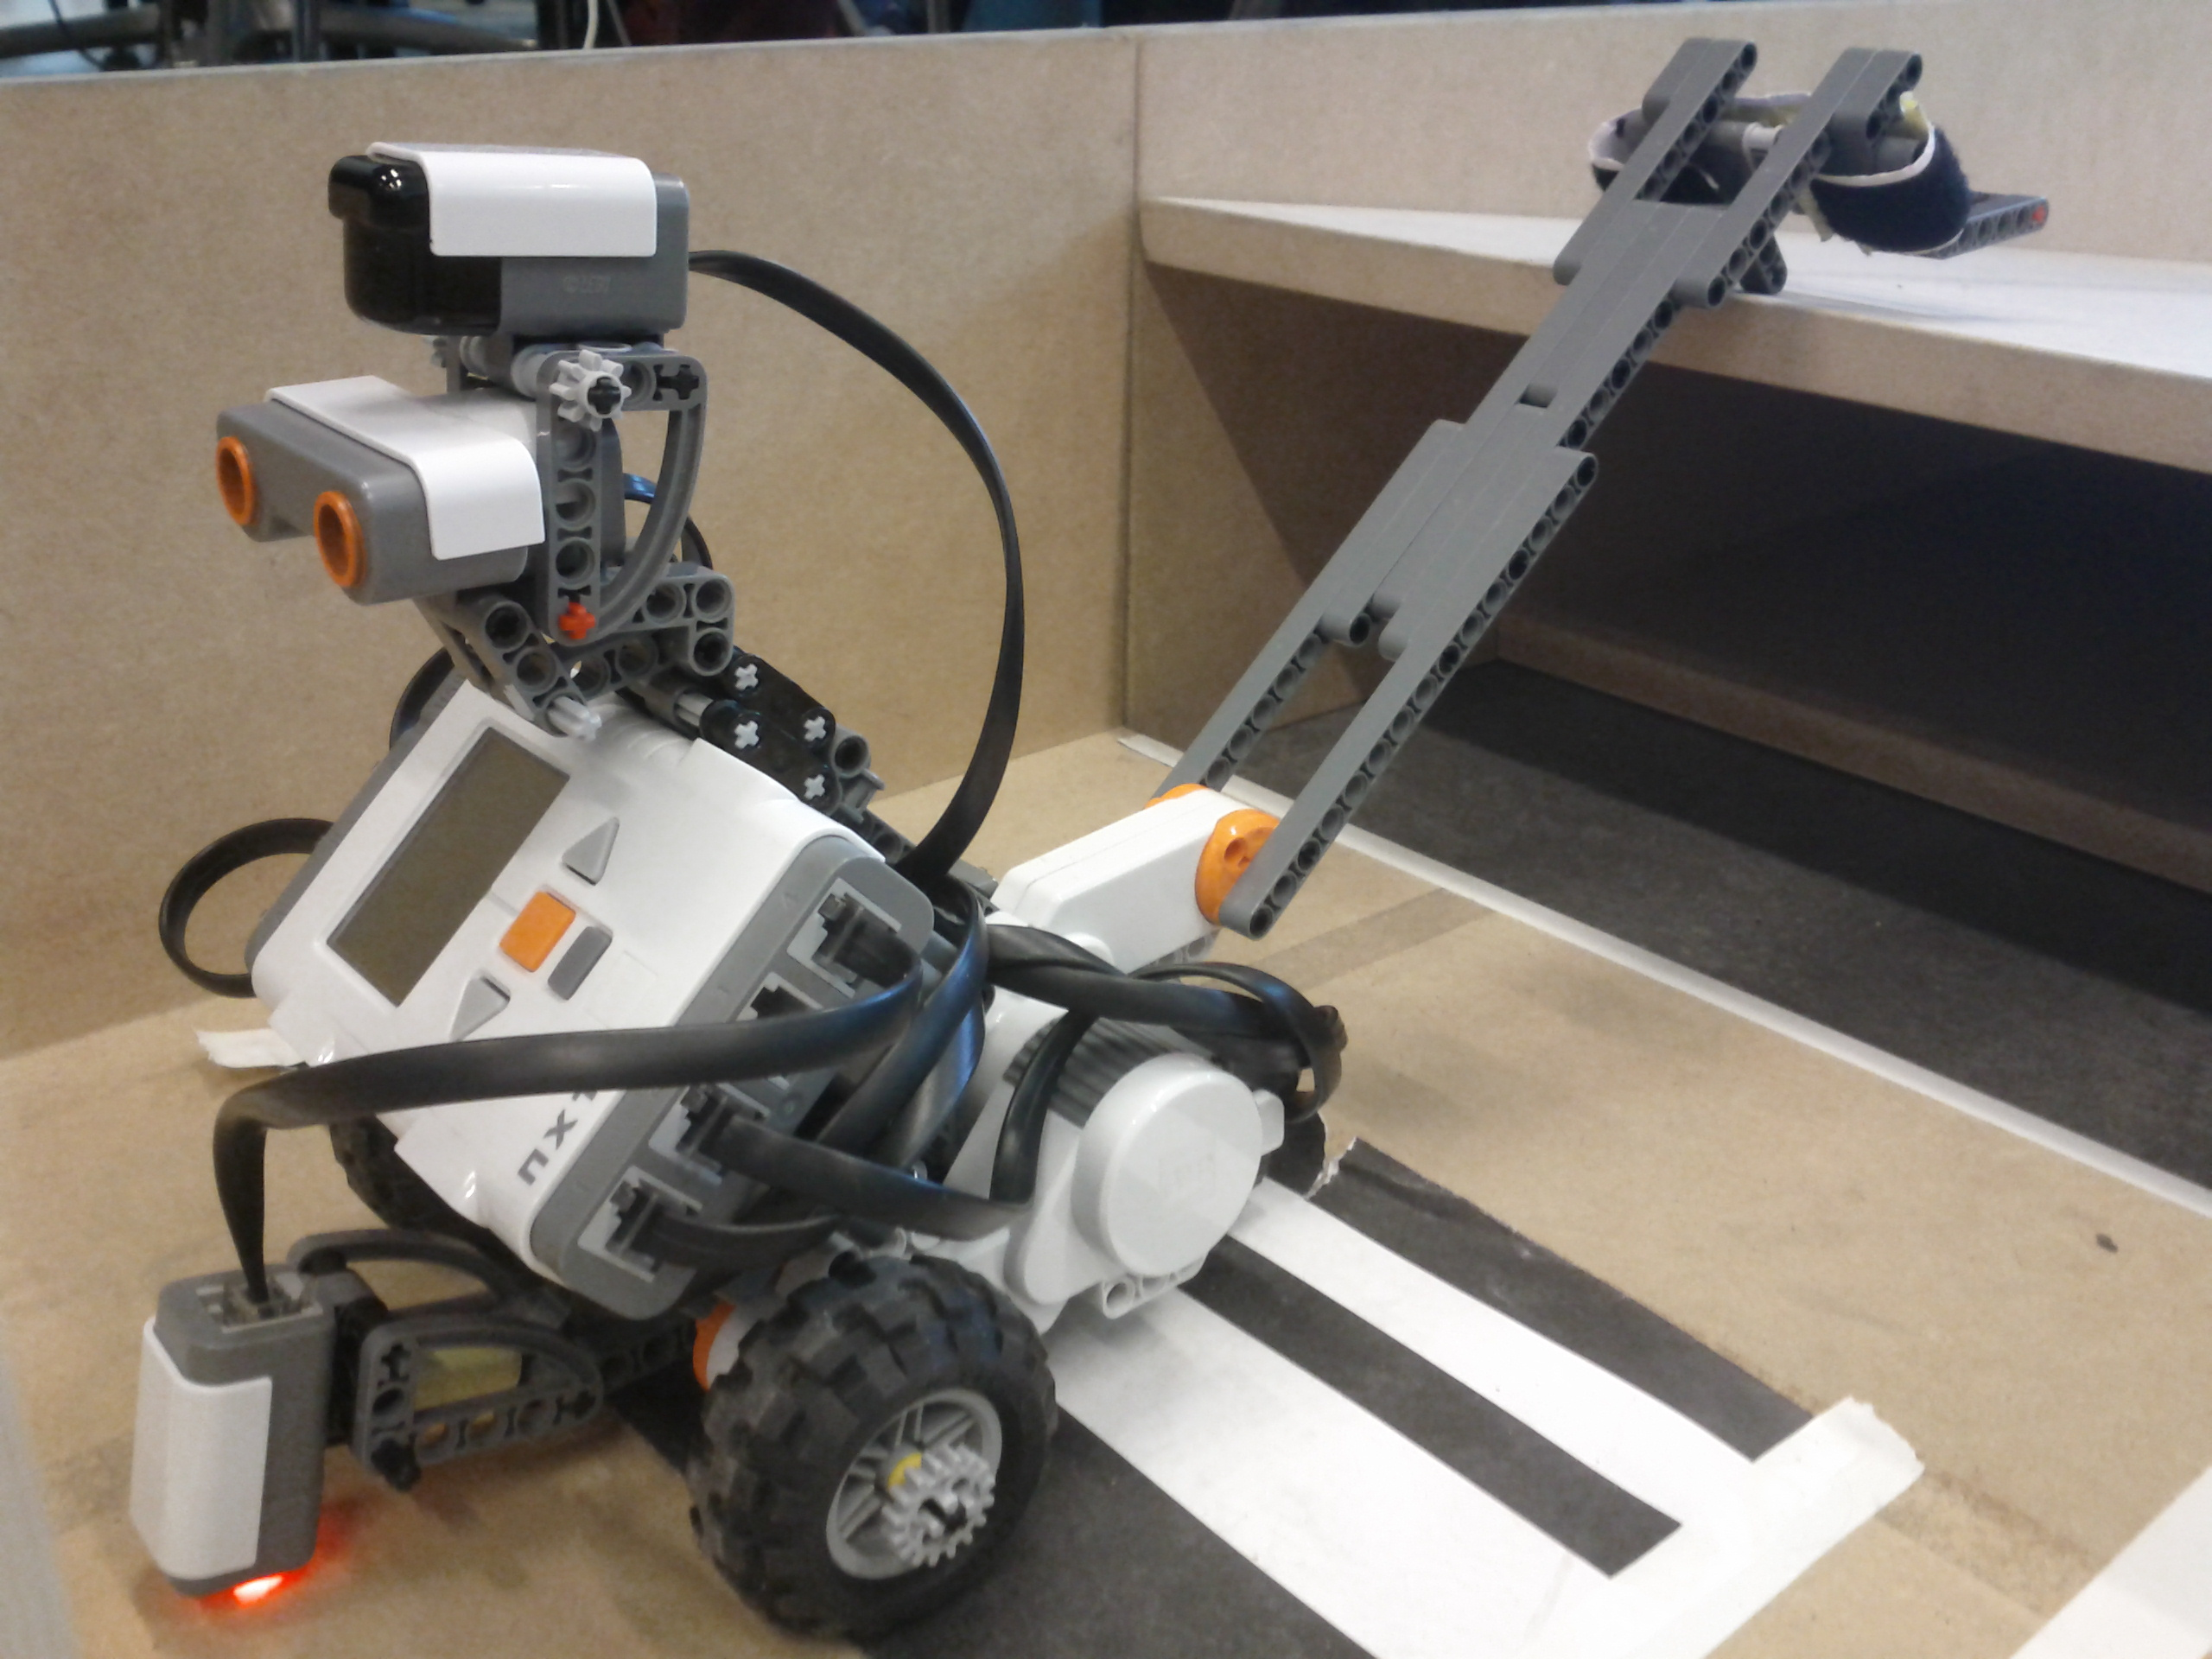
\includegraphics[width=0.52\textwidth]{robotWip}
	\caption{Het openen van een wip}
	\label{fig:robotWip}
\end{figure}


% = voorwerp = %
\subsubsection{Voorwerp} %
\label{sssec:AlgoZoek}
De robot kan het voorwerp vinden door de doolhof te verkennen. In de loop van het eerste semester werd hiervoor een algoritme ontwikkeld dat werd geoptimaliseerd in volgende stappen: 

\begin{enumerate}
\item basisalgoritme: draai bij elke tegel vier keer (eindig in startori\"entatie) en neem de laatste tegel in de queue als volgende tegel;
\item neem de buur die met het minst aantal rotaties bereikt kan worden als volgende tegel.
\item draai bij elke tegel slechts drie keer (eindig niet meer in startori"entatie);
\item kijk muren die vanuit een naburige tegel reeds gedetecteerd werden niet nog eens na;
\item tegels waarvan de vier zijden al gekend zijn en die niet van het type `straight' zijn, worden niet meer bezocht, deze kunnen immers geen barcode bevatten. Het levert geen extra informatie op om de tegel te bezoeken.
\end{enumerate}

Testresultaten van deze optimalisaties worden beschreven in het verslag van vorig semester~\cite{Verslag1}.\\

Bij de start van het tweede semester werd een extra optimalisatie (optimalisatie 6) ontwikkeld. Deze geeft prioriteit aan `dead-ends'. Een voorwerp kan zich immers enkel bevinden op een `dead-end', voorafgegaan door een `straight' met een barcode. Onderstaande testen tonen echter aan dat deze optimalisatie in de meeste gevallen niet effici\"ent is. De optimalisatie werd daarom niet ge\"implementeerd.\\

Nadat het voorwerp gevonden is, wacht de robot tot hij zijn teamgenoot kent. Zo hindert hij de andere robots zo weinig mogelijk.

\subparagraph{Testresultaten van optimalisatie 6}
\label{par:AlgoZoekTest}
De optimalisatie werd getest door de simulator verschillende keren door vier verschillende doolhoven te laten rijden. Een van de testdoolhoven wordt weergegeven in figuur~\ref{fig:TestDead}. De robot startte in elke hoek van elke doolhof zowel zonder optimalisatie als met. De robot dient de tegel met het voorwerp niet te bezoeken; het is voldoende de barcode ervoor te lezen om te weten of het om het juiste voorwerp gaat. Dit heeft als gevolg dat enkel de afgelegde afstand van het startpunt tot de punten~A,~B, C~en~D van belang is. Tabellen~\ref{tab:resultVerken1} en~\ref{tab:resultVerken2} geven resultaten weer voor het doolhof uit figuur~\ref{fig:TestDead}. Niet alle testresultaten worden weergegeven; het groot aantal tabellen zou weinig meerwaarde bieden.\\

\begin{table}[h]
\begin{center}
    \begin{tabular}{ c | c | c | c | c}
   \multicolumn{2}{c|}{Zonder optimalisatie 6} & \multicolumn{2}{|c|}{Met optimalisatie 6} & \\
     gevonden locatie & afgelegde weg (cm) & gevonden locatie &  afgelegde weg (cm) & verbetering?\\ \hline\hline
    B & 880 & A & 720 & ja \\ \hline
    D & 2960 & B & 1520 & ja \\ \hline
    C & 4520 & D & 4320 & ja\\ \hline
    A & 5920 & C & 6120 & nee\\
    \end{tabular}
    \caption{Testresultaten optimalisatie 6: start linksboven in het doolhof uit figuur \ref{fig:TestDead}}
    \label{tab:resultVerken1}
\end{center}
\end{table}

\begin{table}[h]
\begin{center}
    \begin{tabular}{c | c | c | c | c}
   \multicolumn{2}{c|}{Zonder optimalisatie 6} & \multicolumn{2}{|c|}{Met optimalisatie 6} &\\
     gevonden locatie &  afgelegde weg (cm) & gevonden locatie &  afgelegde weg (cm)& verbetering?\\ \hline\hline
    D & 120 & D & 120 & -\\ \hline
    A & 2600 & A & 2920 & nee\\ \hline
    B & 3240 & B & 3720 & nee\\ \hline
    C & 6000 & C & 6240 & nee\\
    \end{tabular}
    \caption{Testresultaten optimalisatie 6: start rechtsonder in het doolhof uit figuur \ref{fig:TestDead}}
    \label{tab:resultVerken2}
\end{center}
\end{table}

\begin{figure}[!h]
\centering
	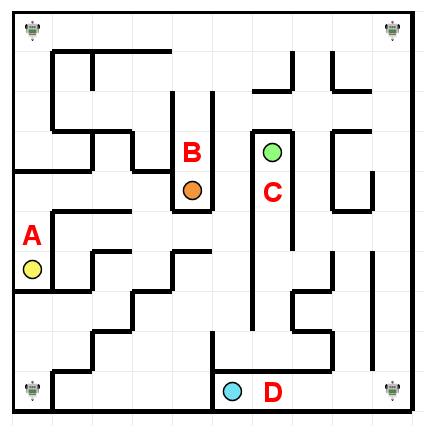
\includegraphics[scale=0.5]{doolhof3}
	\caption{Een van de doolhoven waarop de optimalisatie 6 getest werd}
\label{fig:TestDead}
\end{figure}

%testresultaten: 25x beter (24,3%); 30x even goed (29,1%); 48x slechter (46,6%)
Een vergelijking van alle testresultaten toont dat het algoritme met deze optimalisatie slechts in~$24\%$ van de gevallen een verbetering is. In~$29\%$ van de gevallen levert de optimalisatie geen verschil en in~$47\%$ van de gevallen doet de robot er zelfs langer over. Het is immers moeilijk het kortste pad naar de voorwerplocatie te bepalen wanneer de tegels op dat pad nog niet verkend zijn. In dat geval kan het pad enkel op basis van de \textit{Manhattanafstand} geschat worden, zonder de muren in rekening te brengen. Dit zorgt ervoor dat de robot vaak moet terugkeren om een nieuw pad te zoeken. De optimalisatie is daarom niet geschikt om toe te voegen aan het algoritme.

\subparagraph{Het oprapen van een voorwerp}
Een voorwerp ligt tegen de achterste muur van een `dead-end' tegel. De aanliggende tegel bevat een barcode die het voorwerp identificeert. Dit algoritme wordt uitgevoerd wanneer de robot vlak achter de barcode staat. De robot draait $180\degree$ om zijn as, laat zijn schep volledig naar beneden zakken en rijdt $20$~cm achterwaarts. Zo wordt het voorwerp geklemd tussen de muur en de schep. Klittenband op de schep en het voorwerp zorgt ervoor dat het voorwerp op de schep blijft liggen. De robot rijdt $30$~cm vooruit zodat hij voorbij de barcode staat. Vervolgens aligneert hij zich op de volgende witte lijn.

\subsubsection{Andere robot}
\label{sssec:AlgoCollision}
Een hybride sensor maakt gebruik van een \textit{Wereldsimulator}.
Deze heeft kennis van de posities van andere robots,
gebaseerd op de informatie die de robots doorsturen.
Wij hebben ervoor gekozen geen gebruikt te maken van de hybride sensor; de ultrasone sensor is even geschikt en minder afhankelijk van de communicatiemogelijkheden van andere robots.

De robot houdt tijdens het rijden bij hoeveel afstand hij nog moet afleggen. Wanneer de ultrasone sensor een waarde geeft die kleiner is dan deze afstand, ziet hij een andere robot voor zich. Eerdere metingen toonden immers dat de robot minstens die afstand zonder problemen zou moeten kunnen afleggen. De robot stopt en rijdt de al afgelegde afstand achterwaarts af. Hij rijdt vervolgens naar een willekeurige onverkende tegel van waaruit hij verder verkent. Enkel wanneer de robot op een wip staat, zal hij blijven staan. Indien alle tegels reeds verkend werden, rijdt de robot naar een willekeurige tegel.

% == Samenwerking == %
\subsection{Samenwerking met de teamgenoot}
\label{ssec:AlgoSamen}

% = samenvoegen = %
\subsubsection{Samenvoegen van doolhoven}
\label{sssec:AlgoMappen}
Wanneer een robot zijn voorwerp gevonden heeft, weet hij bij welk team hij hoort. Hij stuurt vanaf dan regelmatig zijn map door en kijkt of zijn teamgenoot hetzelfde doet.
Wanneer de robot een map ontvangt, gaat hij op zoek naar unieke paren. Dit zijn tegels met een voorwerp en de aangrenzende barcode of tegels met een wip en de aangrenzende barcode. De robot kijkt vervolgens of zijn eigen map dit unieke paar ook bevat. Indien dit niet het geval is, zoekt de robot naar andere unieke paren of wacht hij tot een nieuwe doolhof binnenkomt.

Indien de robot het unieke paar ook in zijn map heeft, kunnen beide mappen worden samengevoegd. E\'en van beide overeenkomende punten van de paren wordt als referentiepunt gekozen. Beide mappen worden getransleerd tot hun referentiepunt in de oorsprong ligt. De robot vergelijkt dan de co\"ordinaten van het andere punt uit het unieke paar. Wanneer deze in de twee mappen niet gelijk zijn, wordt de tweede map geroteerd tot deze wel gelijk zijn. De eerste map wordt opnieuw naar zijn oorspronkelijke positie getransleerd. De transformatiematrix die hiervoor nodig is, wordt ook toegepast op de tweede map. Zij ligt nu samen met de eerste.\\ \\
De algemene transformatiematrix bestaat dus uit drie delen:
\begin{itemize}
	\item De translatie van de tweede map naar de oorsprong;
	\item De rotatie van de tweede map;
	\item De translatie van de tweede map naar de oorspronkelijke positie van de eerste map.
\end{itemize}

Deze transformatiematrix verandert echter alleen de co\"ordinaten van de tegels. De tegels moeten ook afzonderlijk de juiste ori\"entatie krijgen. Deze wordt ook verkregen uit het unieke paar. Stel dat `Dead-end.N' overeen komt met `Dead-end.S', dan komt `N' dus overeen met `S' en bijgevolg `E' met `W', `S' met `N' en `´W' met `E'.\\

Wanneer de volledige projectie bepaald is, worden de mappen samengevoegd. Vanaf dat moment is er een pad berekenbaar dat naar de teamgenoot leidt. Dit pad wordt genomen en er wordt niet meer naar verdere updates van de map gekeken. De positie van de andere robot wordt met dezelfde projectie `vertaald' naar een positie in de samengevoegde map.

% = teamgenoot = %
\subsubsection{Teamgenoot bereiken}
\label{sssec:AlgoTeam}

De scheidsrechterscommissie besloot dat alle robots informatie doorsturen over hun positie. Een robot stuurt naar zijn teamgenoot ook zijn map.\\

De robot bepaalt het kortste pad naar de positie van de andere robot volgens een algoritme op basis van $A^{*}$. Hij legt \'e\'en stap van dit pad af en herbekijkt de positie van de andere robot. Indien deze zich verplaatst heeft, wordt het pad opnieuw berekend.

Het zou kunnen dat beide robots in een lus bewegen waardoor ze steeds op dezelfde afstand van elkaar blijven. Om dit te vermijden wordt bij elke stap de lengte van het pad bepaald. Indien deze lengte niet daalde ten opzichte van de vorige stap, blijft de robot een willekeurige periode tussen de nul en tien seconden wachten. Zo wordt vermeden dat de robots niet opnieuw in dezelfde lus komen.


% == SOFTWARE == %
\section{Software}
\label{sec:Softw}
De software bestaat uit twee delen: een project dat op de \textsc{NXT} van de robot loopt en een project dat op de computer loopt (sectie~\ref{ssec:Sdesign}). De \textit{Graphical User Interface (GUI)} laat toe de robot te besturen en de reacties van de robot weer te geven (sectie~\ref{ssec:GUI}). Robots kunnen met elkaar communiceren via \textsc{RabbitMQ} (sectie~\ref{ssec:RabbMQ}). Het is ook mogelijk met gesimuleerde robots te werken (sectie~\ref{ssec:Sim}). Tijdens het verkennen wordt een map opgeslagen van de wereld (sectie~\ref{ssec:Mapping}).\\

Voor volgende secties wordt verwezen naar het verslag van het eerste semester~\cite{Verslag1}. Deze implementaties en ontwerpen werden zonder aanpassingen opnieuw gebruikt:

\begin{itemize}
\item Commando's doorgeven;
\item Bluetooth;
\item Robot.
\end{itemize}

% -- Ontwerp -- %
\subsection{Algemeen software-ontwerp}
\label{ssec:Sdesign}
Figuur~\ref{fig:klasSoft} toont een schematische voorstelling van de belangrijkste klassen in het computerproject. Om de figuur niet te overbelasten, worden methodes niet weergegeven.\\

% klassendiagramma
\begin{figure}[h]
\centering
		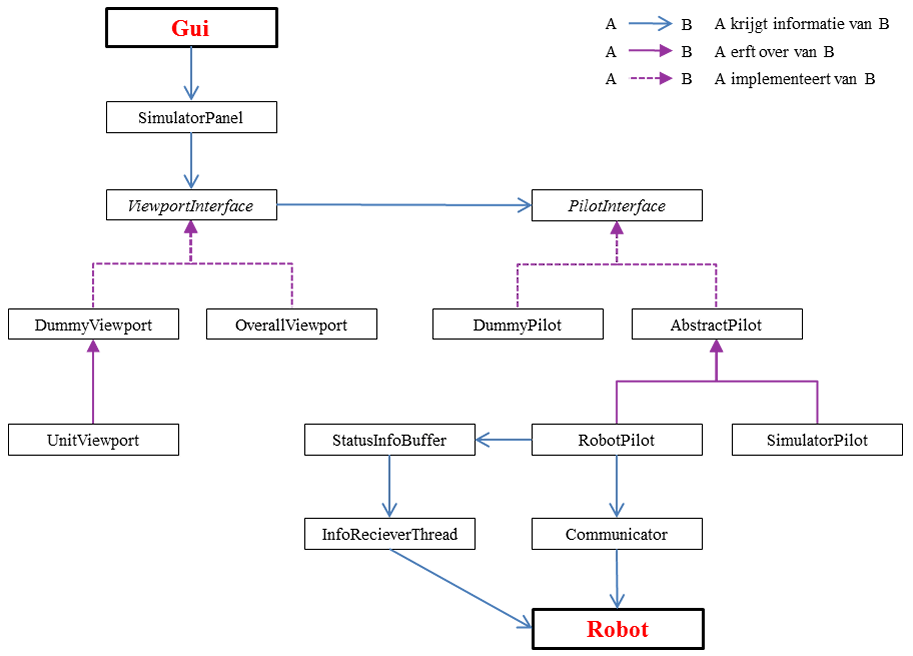
\includegraphics[width=0.95\textwidth]{KlasSoftware}
\caption[Structuur van computerproject]{Schematische voorstelling van de belangrijkste klassen van het computerproject}
\label{fig:klasSoft}
\end{figure}

De \textit{Main}-methode bevindt zich in de \textit{GUI}-klasse. Deze maakt een \textit{SimulatorPanel}-object aan, een overkoepelend panel dat meerdere \textit{Viewports} bevat. Een \textit{OverallViewport} geeft het volledige doolhof met alle robots weer. Dit kan uiteraard enkel wanneer een gekend virtueel doolhof gebruikt wordt en wanneer van alle robots genoeg informatie beschikbaar is. Een \textit{UnitViewport} geeft de wereld van \'e\'en robot (eventueel gesimuleerd) weer: de sensorwaarden en de muren die hij reeds ontdekt heeft. Een wereld waarvan niets geweten is, kan niet worden weergegeven. Dit is het geval voor robots van andere teams: zij worden niet weergegeven in de GUI, met uitzondering van de teamgenoot. Deze laatste stuurt wel zijn map door, maar niet zijn sensorwaarden en wordt gerepresenteerd door een \textit{DummyViewport}. Het aantal \textit{Viewports} hangt af van het aantal gekende werelden.\\

Een \textit{DummyViewport} is aanvankelijk leeg. Wie de teamgenoot van de robot is, wordt immers pas bekend wanneer beide leden van het team hun voorwerp gevonden hebben. Op dat moment zal de \textit{DummyViewport} iets weergeven.\\

Elke \textit{Viewport} krijgt een eigen \textit{Pilot} toegewezen (behalve \textit{OverallViewport}, die krijgt er meerdere). Een \textit{Pilot} is een implementatie van \textit{PilotInterface}. Er zijn verschillende soorten \textit{Pilots}. De keuze van \textit{Pilot} hangt af van het type robot:

\begin{enumerate}
	\item Een robot waarvan de wereld niet kan worden voorgesteld, krijgt geen \textit{Pilot};
	\item Een teamgenoot (die we niet zelf simuleren) heeft een \textit{DummyPilot}. Deze bevat enkel `getters', want deze robot kan niet worden aangestuurd;
	\item Een robot die gesimuleerd wordt, heeft een \textit{SimulatorPilot}. Deze berekent zijn sensorwaarden op basis van een virtuele doolhof;
	\item Een fysieke robot krijgt een \textit{RobotPilot} die via de \textit{Communicator} in verbinding staat met de fysieke robot. De \textit{RobotPilot} krijgt zijn sensorwaarden terug van de robot via de \textit{InfoReceiverThread} en de \textit{StatusInfoBuffer}.
\end{enumerate}

Zowel \textit{SimulatorPilot} als \textit{RobotPilot} erven over van \textit{AbstractPilot}. Dit zijn de `hersenen' van de (gesimuleerde) robot. De \textit{AbstractPilot} bepaalt hoe de (gesimuleerde) robot moet reageren in de gegeven situatie. Ook bouwt de \textit{AbstractPilot} een map op terwijl de (gesimuleerde) robot zich voortbeweegt door het doolhof.

% -- GUI -- %
\subsection{Grafische User Interface}
\label{ssec:GUI}

De \textit{GUI} is zeer flexibel. Naast het paneel dat de doolhof en de robot weergeeft, is het mogelijk verschillende extra panelen te openen:


\begin{itemize}
	\item Het informatiepaneel (links);
	\item Het paneel met sensorgrafieken (onderaan);
	\item De \textit{OverallVieuwport} (linker doolhof);
	\item De map die werd samengevoegd met die van de teamgenoot (rechter doolhof).
\end{itemize}

Figuur~\ref{fig:guiAll} toont de \textit{GUI} met deze extra panelen. In dit geval is de teamgenoot nog niet bekend waardoor het kader van de samengevoegde map leeg is.\\

% figuur GUI met extra schermen
\begin{figure}[h]
\centering
	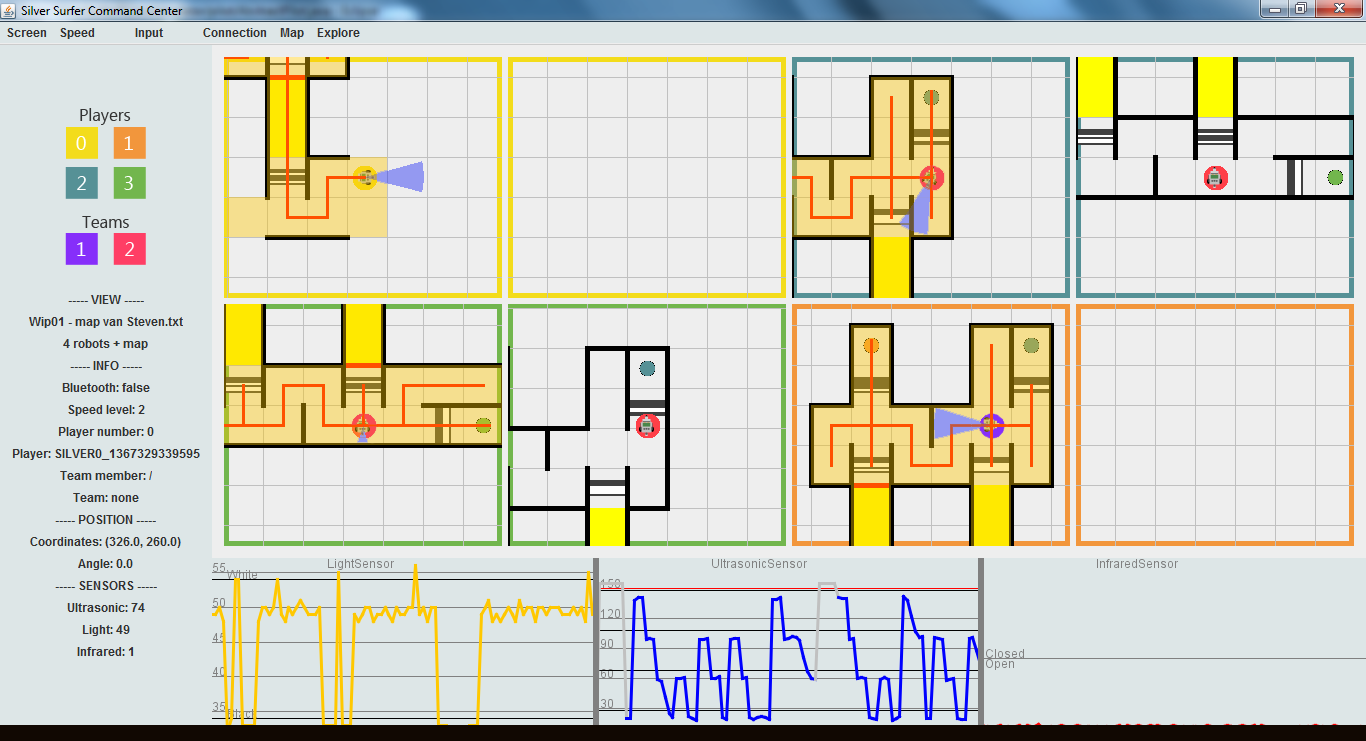
\includegraphics[width=0.7\textwidth]{guiALL}
\caption{De \textit{Graphical User Interface} met extra panelen}
\label{fig:guiAll}
\end{figure}

Wanneer met meerdere robots tegelijkertijd gespeeld wordt, kan voor elke robot een nieuw venster geopend worden. Het is echter ook mogelijk alle robots samen weer te geven, zoals wordt getoond in figuur~\ref{fig:gui4}. Dit is handig bij het testen: alle robots kunnen tegelijkertijd in het oog gehouden worden.

% figuur GUI
\begin{figure}[h]
\centering
	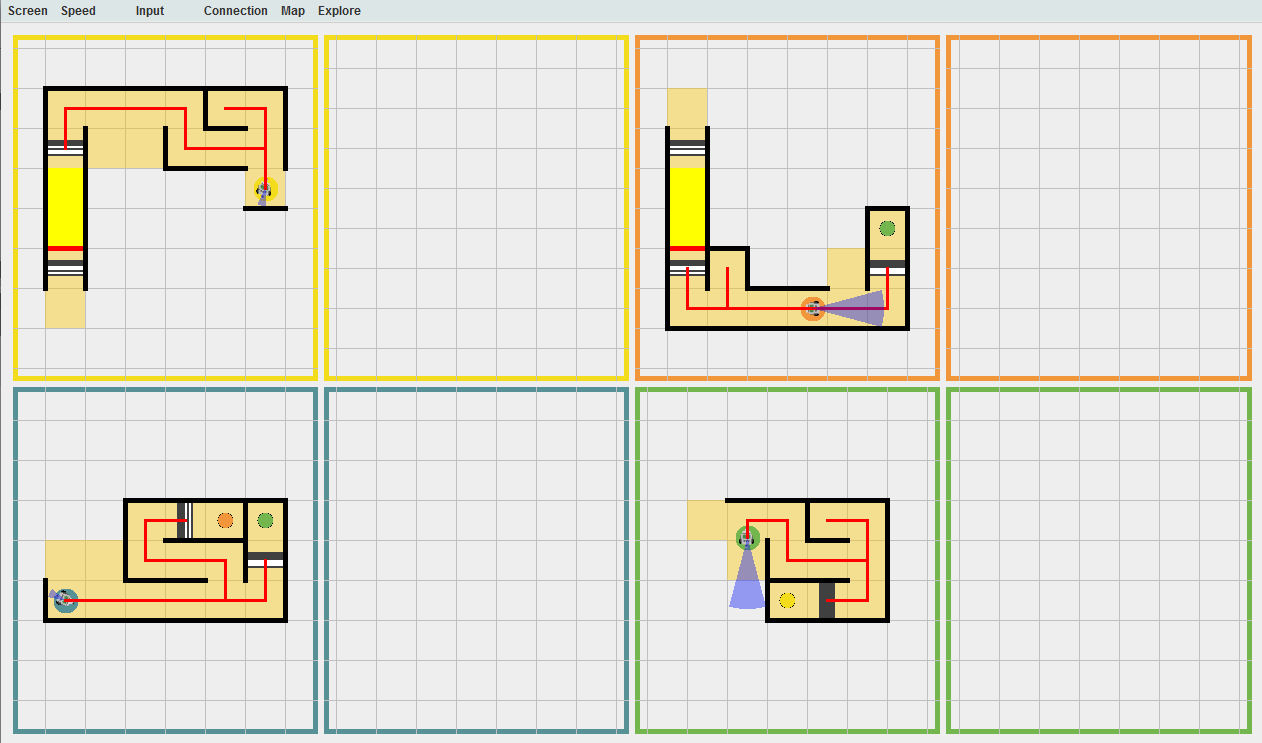
\includegraphics[width=0.7\textwidth]{gui4Robots}
\caption{De \textit{Graphical User Interface} voor vier robots}
\label{fig:gui4}
\end{figure}

Elke robot heeft initieel een eigen kleur: geel, oranje, blauw of groen. Deze kleur hangt af van zijn spelersnummer. Ook zijn voorwerp en de rand van het kader waarin de robot zich bevindt, krijgen deze kleur. Wanneer een robot zijn voorwerp gevonden heeft, verandert zijn kleur in de teamkleur: paars of rood. Wanneer beide teamgenoten hun voorwerp gevonden hebben, voegen ze hun doolhoven samen. De samengevoegde map wordt weergegeven in de rechter kader van elke robot. Figuur~\ref{fig:guiEvolutie} toont deze evolutie in weergave.\\


%TODO moet bij de juiste tekst!!
% klassendiagram HTTTP
\begin{figure}[h]
\centering
	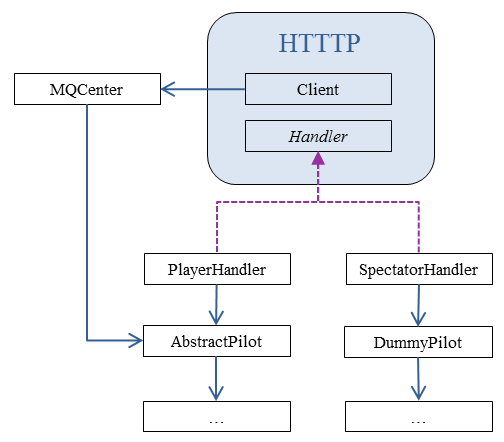
\includegraphics[width=0.45\textwidth]{KlasHTTTP}
\caption{Schematisch overzicht \textit{HTTTP}-klasses}
\label{fig:klasHTTTP}
\end{figure} 

%TODO figuur met samengevoegde map!!
\begin{figure}
\centering
	\begin{subfigure}[h]{0.8\textwidth}
		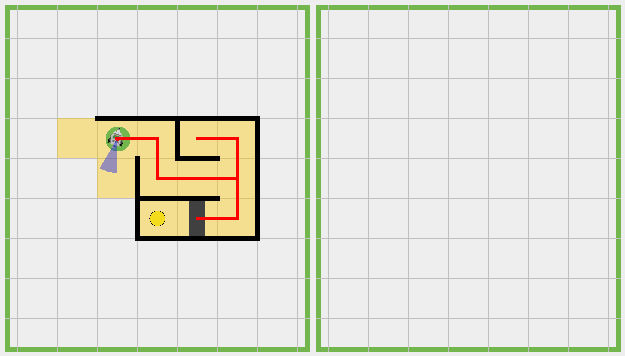
\includegraphics[width=\textwidth]{guiPlayerKleur}
		\caption{Kleur op basis van het spelersnummer}
	\end{subfigure}
	\begin{subfigure}[h]{0.8\textwidth}
		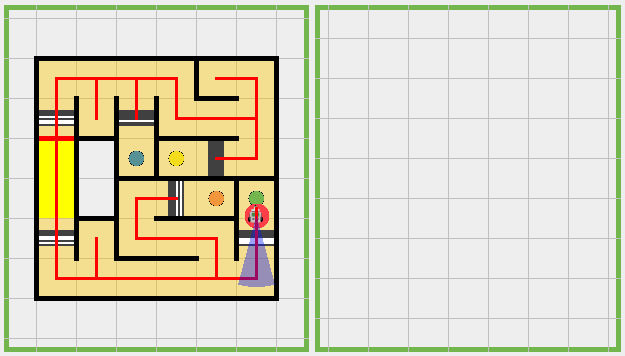
\includegraphics[width=\textwidth]{guiTeamKleur}
		\caption{Kleur op basis van het teamnummer}
	\end{subfigure}
	\begin{subfigure}[h]{0.8\textwidth}
		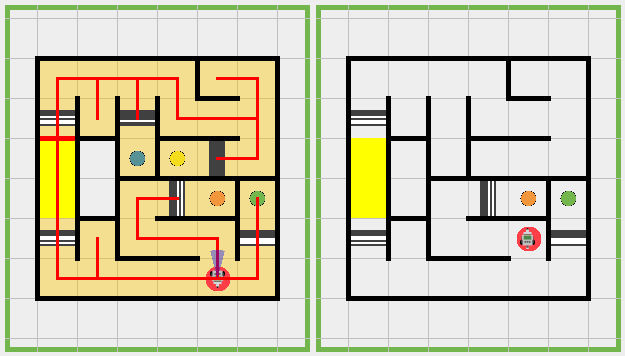
\includegraphics[width=\textwidth]{guiTeamMap}
		\caption{Samengevoegde map}
	\end{subfigure}
	\caption{Evolutie van de \textit{GUI} tijdens het spel}
	\label{fig:guiEvolutie}
\end{figure}

Het pad dat de robot aflegt, geeft de \textit{GUI} weer als een rode lijn. De huidige positie en de huidige ori\"entatie van de robot worden weergegeven door een figuur die draait met de ori\"entatie. Het bereik van de ultrasone sensor wordt grafisch weergegeven met een blauwe boog. Een \textit{DummyViewport} geeft geen sensorwaarden weer. De map-in-opbouw wordt weergegeven op basis van de map die de \textit{Pilot} opstelt. Alle tegels die in de map zitten worden oranje gekleurd. De robot heeft deze tegels niet altijd bezocht, maar weet wel van hun bestaan af. Een wip wordt voorgesteld door een gele strook van twee tegels lang. De kant die omhoog staat wordt aangeduid met een rode lijn.

% -- RabbitMQ -- %
\subsection{Communicatie tussen de robots}
\label{ssec:RabbMQ}



De scheidsrechterscommissie ontwikkelde \textit{Het Team Treasure Trek Protocol (HTTTP)} en een implementatie ervan. De implementatie bevat o.a. een \textit{Client}-klasse die het gebruik van \textsc{RabbitMQ} bijna volledig abstraheert. Ook een \textit{Handler}-interface is voorzien. Deze moet door de teams zelf ge\"implementeerd worden. Figuur~\ref{fig:klasHTTTP} toont een schema van de implementatie.\\

Het computerproject bevat een \textit{PlayerHandler} en een \textit{SpectatorHandler}, om respectievelijk in de \textit{AbstractPilot} en de \textit{DummyPilot} met informatie om te gaan. Een onderscheid is nodig omdat \textit{DummyPilots} `aangestuurd' worden via hun \textit{Handler}.\\

Bij het aanmaken van een \textit{Pilot} wordt een \textit{MQCenter} aangemaakt met bijhorende \textit{Handler}. Het \textit{MQCenter} abstraheert de \textit{Client}-klasse nog verder.

% -- Simulator -- %
\subsection{Simulator} 
\label{ssec:Sim}
De simulator bootst de werking van de robot virtueel na.
Hij kan dezelfde commando's uitvoeren als de werkelijke robot en
genereert sensorwaarden die overeenkomen met die van een fysieke
robot in dezelfde situatie. De simulator is zeer handig bij het testen van algoritmes.

Het genereren van de sensorwaarden gebeurt op basis van een ingeladen map en van de \textit{Wereldsimulator}. De simulator bepaalt zijn positie ten opzichte van de map: hoe ver hij zich van een muur bevindt en op welke ondergrond hij staat. De simulator bepaald bovendien via de \textit{Wereldsimulator} of er zich andere robots in de buurt bevinden en past de ultrasone sensor hieraan aan. Dit is steeds een benadering: de \textit{Wereldsimulator} weet enkel op welke tegel een robot zich bevindt. Hij heeft geen kennis van de positie ten opzichte van die tegel. Op de berekende sensorwaarde wordt steeds een ruis toegepast. Dit om de onnauwkeurigheid van de metingen van de fysieke sensoren in rekening te brengen.

%TODO dit is te gedetailleerd, niet?
%Om de ultrasone sensor te simuleren maken we gebruik van de geladen map, om de afstand tot muren te berekenen en van de \textit{Wereldsimulator}, om de afstand tot andere robots te simuleren. Uit de informatie in de geladen map en de posities van de andere robots wordt een verzameling van obstakels opgesteld (in java Rectangle2D objecten). Voor de berekening van de afstand wordt een voorstelling van de `conus' van de ultrasone sensor opgesteld (in java Arc2D). De `conus' wordt in een lus telkens groter gemaakt, dan gebruiken we de `intersect'-methode van Arc2D op elk obstakel, de eerste keer dat er een `intersection' gedetecteerd wordt is de straal van de Arc2D gelijk aan de te simuleren afstand.

Op de bewegingen van de simulator wordt geen ruis toegevoegd.
Wanneer de fysieke robot zich regelmatig aligneert,
rijdt hij immers nauwkeurig genoeg.


% -- Mapping -- %
%TODO beter titel? Moeten ons houden aan de titels van de template van de commissie
\subsection{Mappen van een doolhof}
\label{ssec:Mapping}
Het \textit{Mapping}-pakket bevat objecten die elementen uit de wereld van een robot voorstellen. Figuur~\ref{fig:klasMap} geeft de structuur van het pakket weer. De klasse \textit{MapGraph} brengt al deze elementen samen. Ze biedt functionaliteiten om van de huidige tegel naar een aanliggende tegel te reizen en om de map dynamisch uit te breiden. Elke \textit{Tile} wordt via \textit{Edges} verbonden met zijn buurtegels. Zo wordt impliciet een hele graaf bijgehouden. De klasse \textit{MapReader} kan uit een bepaald text-bestand een \textit{MapGraph} opstellen.\\

De \textit{SimulatorPilot} heeft een \textit{MapGraph} die de virtuele doolhof voorstelt. Tijdens het verkennen wordt een nieuwe \textit{MapGraph} opgesteld door de \textit{AbstractPilot}. Deze bevat enkel informatie die de robot zelf verzamelde.


% klassendiagram mapping
%\begin{figure}[h]
%TODO vlakbij de tekst zetten in de pdf
% klassendiagram mapping
\begin{figure}[h!]
\centering
	\includegraphics[width=0.65\textwidth]{klasMapping}
\caption{Klassendiagram mapping}
\label{fig:klasMap}
\end{figure}

%\begin{figure}

%\centering
%	\includegraphics[width=0.8\textwidth]{klasMapping}
%\caption{Klassendiagram mapping}
%\label{fig:klasMap}
%\end{figure}

%\begin{figure}
%\centering
%\begin{tikzpicture}[thick,scale=0.7, every node/.style={scale=0.7}]
%\tikzstyle{line} = [draw, -stealth, thick]
%
%\tikzstyle{block} = [draw, rectangle, text width=8em, text centered, minimum height=15mm, node distance=7em, rounded corners]
%\node [block] (Tile) {Tile};
%\node [block, left of=Tile, xshift=-5em] (Edge) {Edge};
%\node [block, above of=Tile, yshift=3em] (MapGraph) {MapGraph};
%\node [block, above of=MapGraph, yshift=3em]
%(PilotInterface) {PilotInterface};
%\node [block, above of=PilotInterface, yshift=3em]
%(not) {...};
%\node [block, right of=Tile, xshift=5em] (TileContent) {TileContent};
%\node[block , below of=Edge, yshift=-3em](Obstruction){Obstruction};
%\node [block, below of=TileContent, yshift=-3em] (Barcode) {Barcode};
%\node [block, right of=Barcode, xshift=3em]
%(TreasureObject) {TreasureObject};
%\node [block, left of=Barcode, xshift=-3em]
%(Seesaw) {Seesaw};
%
%%arrows
%\path [line, line width=1.6pt] (Edge) -- (Tile);
%\path [line, line width=1.6pt] (TileContent) -- (Tile);
%\path [line, line width=1.6pt] (Tile) -- (MapGraph);
%\path [line, line width=1.6pt] (MapGraph) -- (PilotInterface);
%\path [line, line width=1.6pt] (PilotInterface) -- (not);
%\path [line, line width=1.6pt] (Obstruction) -- (Edge);
%
%\path [line, color=blue, line width=1.6pt] (Seesaw) -- (TileContent);
%\path [line, color=blue, line width=1.6pt] (Barcode) -- (TileContent);
%\path [line, color=blue, line width=1.6pt] (TreasureObject) -- (TileContent);
%%\path [line] (decision1) -| node[yshift=0.5em, xshift=-10em] {no} (process2);
%\end{tikzpicture}
%\caption{Klassendiagram mapping, de blauwe pijlen wijzen op overerving}
%\label{fig:klasMap}
%\end{figure}

% == BESLUIT == %
\section{Besluit}
\label{sec:Besluit}
De bouw van de robot bevat een lange schep, voorzien van klittenband. De schep kan via een motor gekanteld worden. Wanneer de robot geen andere uitweg heeft, kan deze eventueel gebruikt worden om een wip te openen. De lichtsensor is gemonteerd op een hefboomsysteem dat omhoog klapt wanneer het de wip raakt. Zo geraakt de robot makkelijk de wip op. De ultrasone sensor en de infraroodsensor zijn vast gemonteerd en kunnen niet bewegen ten opzichte van de robot.\\

Er kunnen verschillende robots worden gesimuleerd of gemodelleerd. Al deze robots hebben een eigen idee van de wereld. Deze verschillende werelden worden weergegeven in de \textit{GUI} via \textit{Viewports}. Een \textit{OverallViewport} toont de werkelijke wereld en alle robots erin.\\

De robot kan via \textsc{RabbitMQ} posities en mappen doorsturen naar en ontvangen van zijn teamgenoot. Door zijn eigen map samen te voegen met die van zijn teamgenoot, kan de robot een pad naar de teamgenoot bepalen. Botsingen met andere robots worden vermeden door de waarde van de ultrasone sensor steeds in het oog te houden.


\newpage
\makeappendix

%% == DEMO 1 == %
\section{Demo 1}
\label{Asec:demo1}
De robot wordt voor de eerste demo voorzien van een schep die bestaat uit een halve wc-rol. De infraroodsensor is ge\"installeerd, maar wordt nog niet gebruikt. Wanneer de robot zijn voorwerp vindt, stuurt hij een bericht via \textsc{RabbitMQ}. De \textit{GUI} is opgesplitst in verschillende \textit{Viewports} die elk een of meerdere \textit{Pilots} weergeven.

% == resulaten == %
\subsection{Resultaten}
\label{Assec:result1}
Het algoritme waarmee de robot zijn voorwerp opraapte doet de robot een verplaatsing maken. De \textit{ExploreMaze}-thread wist echter niet dat de robot van plek was veranderd. In de waan dat de robot op een andere plek stond dan in werkelijkheid, gaf de thread verkeerde instructies waardoor de robot tegen een muur reed.

Het schepsysteem van de robot functioneerde niet. Tijdens de demo faalde de robot toen hij het object moest oprapen. 

% == conclusies == %
\subsection{Conclusies}
\label{Assec:conc1}
Om te vermijden dat de \textit{ExploreMaze}-thread een verkeerd beeld krijgt van de situatie, moeten de algoritmes die de thread onderbreken zorgen dat de robot steeds op dezelfde plek eindigt als waar de thread denkt dat hij staat.
Ook de schep moet worden aangepast. Deze kan van klittenband voorzien worden.

% == aanpassingen == %
\subsection{Oplijsting aanpassingen verslag}
\label{Assec:aanp1}
Volgende secties werden aangepast ten opzichte van het eerste tussentijds verslag van het tweede semester:

% overzicht aangepaste secties
\begin{itemize}
\item \textit{Samenvatting:} aangepast.
\item \textit{\ref{ssec:Bouw} Fysieke bouw:} de schep vooraan.
\item \textit{\ref{sssec:AlgoZoek} Zoeken van het voorwerp:} testen van de prioriteit.
\item \textit{\ref{sssec:AlgoCollision} Weg vinden naar teamgenoot:} nieuwe sectie.
%\item \textit{\ref{ssec:AlgoMappen} Twee mappen samenvoegen:} nieuwe sectie.
\item \textit{\ref{ssec:GUI} Grafische User Interface:} nieuwe figuren en aangepaste tekst.
\item \textit{\ref{ssec:RabbMQ} Communicatie via RabbitMQ:} implementatie \textit{HTTTP}.
\item \textit{\ref{ssec:Mapping} Mappen van een doolhof:} wip en voorwerpen toegevoegd.
\end{itemize}

%% == DEMO 2 == %
\section{Demo 2}
\label{Asec:demo2}
De bouw van de robot wordt uitgebreid met een infraroodsensor. De schep vooraan wordt aangepast en van klittenband voorzien. Zowel de schep als de lichtsensor zijn gemonteerd op een hefboomsysteem dat omhoog klapt wanneer het de wip raakt. Omdat het rijden over een wip onnauwkeurigheden introduceert, wordt dit zoveel mogelijk vermeden tijdens het verkennen.

% == resulaten == %
\subsection{Resultaten}
\label{Assec:result2}
Het verkennen van het doolhof gebeurde volledig zoals het hoorde. De robot was enkele dagen voor de demonstratie volledig gekalibreerd en reed heel nauwkeurig. Het nemen van de wip is echter niet gelukt omdat de robot bleef haken achter de wip.
De robot slaagde er niet in zijn voorwerp te vinden. De demonstratie was immers al stilgelegd voordat de robot hiertoe de kans had.

De simulatie van vier robots verliep erg goed. Enkel de visualisatie van het pad toonde discontinu"iteiten.

% == conclusies == %
\subsection{Conclusies}
\label{Assec:conc2}
Het rijden over een wip vraagt extra testen zodat eventueel het hefboomsysteem kan worden aangepast. Ook de discontinu\"iteiten in de visualisatie van het pad zouden verholpen moeten worden.

% == aanpassingen == %
\subsection{Oplijsting aanpassingen verslag}
\label{Assec:aanp2}
Volgende secties werden aangepast ten opzichte van het tweede tussentijds verslag van het tweede semester:

%TODO
% overzicht aangepaste secties
\begin{itemize}
\item \textit{\ref{ssec:Bouw} Ontwerp:} nieuwe bouw.
\item \textit{\ref{ssec:Kalib} Kalibratie:} nieuwe sectie.
\item \textit{\ref{sssec:AlgoAllign} De robot aligneren:} nieuw algoritme.
\item \textit{\ref{sssec:AlgoBar} Barcode:} nieuw algoritme.
\item \textit{\ref{sssec:AlgoWip} Wip:} nieuwe sectie.
\item \textit{\ref{sssec:AlgoTeam} Weg vinden naar teamgenoot:} aangepast.
\item \textit{\ref{sssec:AlgoMappen} Twee doolhoven samenvoegen:} nieuwe sectie.
\item \textit{\ref{sssec:AlgoCollision} Botsingen met andere robots vermijden:} nieuwe sectie.
\item \textit{\ref{ssec:GUI} Grafische User Interface:} nieuwe figuren en aangepaste tekst.
\end{itemize}

%% == DEMO 3 == %
\section{Demo 3}
\label{Asec:demo3}
Door de bouw van de robot compacter te maken kan de schep achteraan geplaatst worden en voorzien worden van een motor. Zo wordt het mogelijk eventueel een wip te openen met de schep.

De robot vermijdt andere robots met behulp van zijn ultrasone sensor. De robot kan twee mappen samenvoegen en kan op basis hiervan naar zijn teamgenoot rijden.

% == resulaten == %
\subsection{Resultaten}
\label{Assec:result3}
De demonstratie van de simulator verliep volledig zoals het hoorde: de robots vonden alle vier hun voorwerp en de twee duo's konden deze voorwerpen bij elkaar brengen. De gesimuleerde robots reden hierbij niet tegen elkaar.\\

De fysieke robot was niet in staat robots te vermijden. Het is immers niet zomaar mogelijk de robot te onderbreken in zijn bewegingen. De robot zou echter samen met drie simulatoren zonder deze functie moeten kunnen werken. Er liep echter iets mis tijdens het verkennen waardoor de fysieke robot vast liep.
Het was wel mogelijk het algoritme om de wip te openen te demonstreren.\\

Wanneer met meerdere teams samen gepeeld werd, kwamen enkele verbindingsproblemen aan het licht. Het bleek bovendien dat we een bepaald onderdeel van het protocol verkeerd \\ge\"implementeerd hadden: dit deel was niet lang voor de demo veranderd. Het betrof het doorsturen van posities. Deze posities dienden relatief ten opzichte van de startpositie en ori\"entatie te zijn, maar dit hadden we verkeerd begrepen.

% == conclusies == %
\subsection{Conclusies}
\label{Assec:conc3}
We hadden te weinig tijd robotdetectie te implementeren op de robot zelf. Dit kon niet volledig analoog aan de simulator gebeuren omdat de robot met \textit{threads} werkt die niet zomaar onderbroken kunnen worden. De manier waarop dit wel ge\"implementeerd zou kunnen worden, was volledig uitgewerkt. Het is jammer dat dit niet meer is gelukt.

Er was ook niet genoeg tijd de fysieke robot voldoende te testen op grote doolhoven. Ook het verbinden met andere teams werd onvoldoende getest.

We zijn echter heel tevreden over de simulator en de \textit{GUI}. Deze simulator werkt volledig zoals het hoort en de \textit{GUI} toont alles wat gebeurt in een overzichtelijk veld.

% == aanpassingen == %
\subsection{Oplijsting aanpassingen verslag}
\label{Assec:aanp3}
Volgende secties werden aangepast ten opzichte van het derde tussentijds verslag van het tweede semester:

% overzicht aangepaste secties
\begin{itemize}
	\item \textit{\ref{sssec:AlgoWip} Wip openen:} `locken' uitgelegd, figuur toegevoegd;
	\item \textit{\ref{sssec:AlgoCollision} Andere robot:} correctere uitleg robotdetectie;
	\item \textit{\ref{ssec:GUI} Grafische User Interface:} nieuwe figuren, tekst meer uitgebreid;
	\item \textit{\ref{ssec:Sim} Simulator:} simulatie ultrasone sensor;
	\item \textit{\ref{Asec:demo3} Demo 3:} nieuwe sectie;
	\item \textit{\ref{Asec:beschrijvingProces} Beschrijving van het proces:} nieuwe sectie;
	\item \textit{\ref{Asec:werkverdeling} Beschrijving van de werkverdeling:} nieuwe sectie;
	\item \textit{\ref{Asec:scheids} bijdrage aan de scheidsrechterscommissie:} nieuwe sectie;
	\item \textit{\ref{Asec:kritisch} Kritische analyse:} nieuwe sectie;
\end{itemize}

Deze secties bevatten een aangepaste inhoud ten opzichte van het vorige verslag. Andere secties werden ook aangepast, maar daar ging het enkel om de verwoording van de inhoud.

\section{Beschrijving van het proces}
\label{Asec:beschrijvingProces}

We zijn het semester begonnen met samen de opdracht te lezen en verschillende oplossingen te bespreken. Dit leidde tot een bepaalde strategie \cite{Strategie} die we zouden volgen doorheen het semester. Nadat iedereen wist waar het algemene project heen zou gaan, werkte iedereen vooral aan `zijn/haar' deel van het project. Wanneer nodig werd hulp gevraagd aan andere teamleden.

Er werd steeds in een tabel bijgehouden wie wanneer aan wat had gewerkt. Dit gaf eveneens een zicht op wat er al klaar was en wat nog moest gebeuren. Hoewel af en toe nog werk dubbel gedaan werd, vermijdde het overzicht in deze tabel dit meestal.
De code werd gedeeld via \textit{GitHub}. Voor de \textit{LaTeX}-code gaf dit af en toe problemen, maar verder zorgde \textit{GitHub} er meestal voor dat iedereen steeds de juiste versie van de code had.


\section{Beschrijving van de werkverdeling}
\label{Asec:werkverdeling}
Tabel~\ref{tab:werkuren} geeft weer hoeveel tijd in het project gestoken werd. Figuur~\ref{fig:werkverdeling} toont wie aan welke aspecten van het project heeft gewerkt.
Maxim nam de taak van teamco\"ordinator op zich, Nele die van secretaris. Sophie vertegenwoordigde het team in de scheidsrechterscommissie.

%TODO laatste week aanvullen!!
\begin{table}[h]
\begin{center}
    \begin{tabular}{ r | c  c  c  c  c  c}
     & Nele & Toon & Sam & Sophie & Gerlinde & Maxim \\ \hline
    week 1 & 9u00 & 9u00 & 8u55 & 7u15 & 7u30 & 9u30\\
   	week 2 & 10u00 & 22u10 & 12u00 & 9u00 & 8u30 & 28u00\\
	week 3 & 14u00 & 25u05 & 9u00 & 8u00 & 9u15 & 6u15\\
	week 4 & 16u15 & 14u40 & 13u27 & 9u00 & 14u30 & 20u30\\
	week 5 & 13u00 & 7u45 & 10u00 & 11u15 & 11u00 & 14u00\\
	week 6 & 11u30 & 7u00 & 17u10 & 15u00 & 14u00 & 35u45\\
	week 7 & 13u30 & 14u40 & 15u47 & 12u30 & 12u00 & 20u30\\
	week 8 & 5u00 & 5u00 & 6u00 & 13u37 & 10u00 & 27u45\\
	week 9 & 5u00 & 5u15 & 6u00 & 7u30 & 11u30 & 5u00\\
	week 10 & 14u30 & 7u40 & 6u30 & 6u30 & 11u45 & 16u00\\
	week 11 & 13u00 & 13u20 & 7u10 & 13u30 & 7u50 & 22u00\\ \hline
	totaal & 124u45 & 131u55 & 112u00 & 114u07 & 117u50 & 205u15 \\
	gemiddeld & 11u20 & 12u00 & 10u11 & 10u22 & 10u43 & 18u40
    \end{tabular}
    \caption{Overzicht werkuren (week 8 bevat ook de uren van de paasvakantie)}
    \label{tab:werkuren}
\end{center}
\end{table}

\begin{figure}[h]
        \centering
        \begin{subfigure}[hb]{0.15\textwidth}
                \centering
                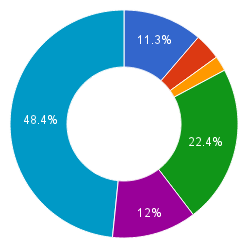
\includegraphics[width=\textwidth]{werk_Nele}
                \caption{Nele}
        \end{subfigure}%
        \begin{subfigure}[hb]{0.15\textwidth}
                \centering
                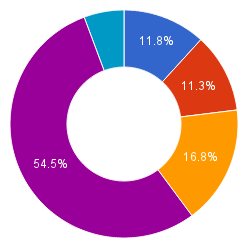
\includegraphics[width=\textwidth]{werk_Toon}
                \caption{Toon}
        \end{subfigure}%
        \begin{subfigure}[hb]{0.15\textwidth}
                \centering
                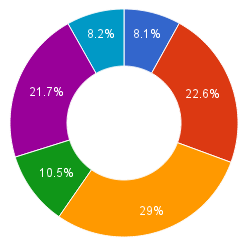
\includegraphics[width=\textwidth]{werk_Sam}
                \caption{Sam}
        \end{subfigure}%
        \begin{subfigure}[hb]{0.15\textwidth}
                \centering
                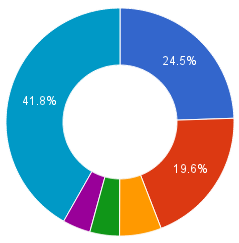
\includegraphics[width=\textwidth]{werk_Sophie}
                \caption{Sophie}
        \end{subfigure}%
        \begin{subfigure}[hb]{0.15\textwidth}
                \centering
                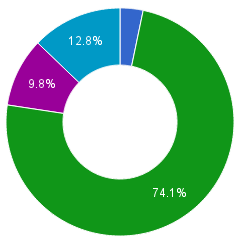
\includegraphics[width=\textwidth]{werk_Gerlinde}
                \caption{Gerlinde}
        \end{subfigure}%
        \begin{subfigure}[hb]{0.15\textwidth}
                \centering
                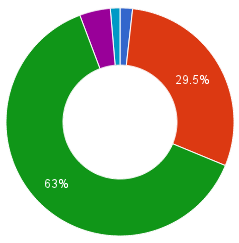
\includegraphics[width=\textwidth]{werk_Maxim}
                \caption{Maxim}
        \end{subfigure}%
        \begin{subfigure}[hb]{0.11\textwidth}
                \centering
                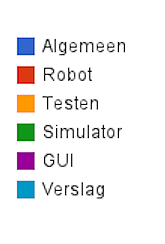
\includegraphics[width=\textwidth]{werk_legende}
                \caption{legende}
        \end{subfigure}
 \caption{Weergave van de werkverdeling}
\label{fig:werkverdeling}
\end{figure}

\section{Bijdrage aan de scheidsrechterscommissie}
\label{Asec:scheids}
De vergaderingen van de scheidsrechterscommissie hadden als doel met alle teams samen een invulling aan het project te geven. Elke vergadering werd een andere voorzitter en secretaris aangewezen. Dit gaf soms problemen omdat niet alle voorzitters ervaring hadden met het leiden van vergaderingen. Discussi\"eren werd dan moeilijk: niet iedereen kreeg de kans te spreken, sommigen gaven ongefundeerde argumenten en soms werd te lang gediscussieerd over een klein detail. Een praktische informatiesessie over vergaderen kan hier misschien uitkomst bieden.

De scheidsrechterscommissie gaf ieder team de kans bij te dragen aan belangrijke beslissingen. Door elk team een afgevaardigde te laten sturen, hoefde niet iedereen zich hiermee bezig te houden. De afgevaardigde diende enkel de mening van zijn team te brengen op de vergadering en het team achteraf in te lichten van de gemaakte beslissingen.\\

Ik, Sophie Marien, vertegenwoordigde team Zilver op de scheidsrechterscommissie. Mijn inbreng bestond uit het idee van de infraroodbal onder de wip om zijn stand te detecteren. Ik heb ook geprobeerd robotdetectie op te lossen via infraroodlichtjes op de robots. Dit werkte uiteindelijk niet omdat de intensiteit van de infraroodlichtjes niet voldeed. Ze werden enkel op korte afstand gedetecteerd waardoor hun nut verviel.
Verder heb ik regelmatig een verslag afgekeurd omdat het onnauwkeurigheden bevatte of omdat ik niet akkoord was met een beslissing.

\section{Reflectie van de oplossingsstrategie}
\label{Asec:strategie}
In de algemene oplossingsstrategie~\cite{Strategie} wordt de opdracht opgedeeld in deelproblemen. De reflectie volgt deze onderdelen.

\paragraph{Hoe vindt de robot zijn voorwerp?}
Het verkenalgoritme werd inderdaad voorzien van een optimalisatie die prioriteit geeft aan `dead-ends'. Uit testen bleek echter dat dit niet tot het verwachte resultaat leidde. De optimalisatie werd daarom weer uit het algoritme gehaald.

Bij het lezen van barcodes voegt de robot automatisch extra muren toe indien dit mogelijk is. Dit is het geval wanneer de barcode een voorwerp aanduidt of een wip. Deze strategie bleek een goed idee. De robot diende zo enkele tegels minder te verkennen.

\paragraph{Hoe raapt de robot het voorwerp op?}
Wanneer het voorwerp werd opgeraapt via een schep achteraan, bleek de robot te lang te zijn om nog goed te kunnen manoeuvreren. De schep werd daarom vooraan geplaatst, zonder de extra motor, maar ook dit bleek niet ideaal te werken. Uiteindelijk werd terug gekeerd naar het oorspronkelijke concept. De robot werd deze keer echter volledig herbouwd en compacter gemaakt waardoor het concept wel haalbaar werd. Dit oorspronkelijke concept was zeker een goed idee. Het concept werd bovendien nog uitgebreid met een extra lange schep die de wip kon openen.

\paragraph{Hoe vindt de robot zijn teamgenoot?}
De scheidsrechterscommissie heeft geen manier voorzien om een gemeenschappelijk punt af te spreken. De robot rijdt daarom gewoon naar de plek waar de andere robot zich op dat moment bevindt. Hij controleert echter regelmatig of hij wel dichter komt. Wanneer beide robots dit doen, komen ze elkaar tegen op het midden van het pad, wat tot hetzelfde resultaat leidt als het oorspronkelijke concept. Het huidige concept is bovendien eenvoudiger aangezien geen tijd wordt verloren met het bepalen van een gemeenschappelijk punt.

\paragraph{Hoe kan de robot over de wip?}
De stand van de wip kon makkelijk bepaald worden via de infraroodsensor, dit was een heel goed idee. De lichtsensor werd op een scharnier geplaatst zodat deze achteruit klapt wanneer de robot de wip raakt. Zo vormt dit geen probleem.

Een extra functionaliteit die werd toegevoegd, bestond in het handmatig openen van de wip. Dit kon aan de hand van de lange schep. Deze functionaliteit werd niet vaak gebruikt tijdens het spel, maar bood een oplossing wanneer de robot volledig ingesloten zit.

\paragraph{Hoe gaat de robot om met foute informatie?}
Wanneer met eigen simulators getest werd, bleek dit geen probleem te zijn: zij stuurden enkel juiste informatie door. Het `grijze muren' systeem was daarom niet nodig. Er is onvoldoende getest met robots van andere teams om te kunnen besluiten dat dit hier een probleem zou zijn.

\section{Kritische analyse}
\label{Asec:kritisch}
Na het eerste semester was de code \'e\'en grote puinhoop. De eerste weken van dit semester werden daarom besteed aan het herordenen en herschrijven van de code die we al hadden. Hier is veel tijd in gekropen, maar het maakte het geheel heel wat overzichtelijker. Later hebben we deze `verloren' tijd hier zeker aan terugverdiend.\\

In de loop van het semester werd de bouw van de robot volledig veranderd. We zagen tijdens de eerste demo en bij de testen dat de robot zeer onstabiel was. Het nieuwe ontwerp is stabieler, robuuster en nauwkeuriger. Het was een goede beslissing het ontwerp volledig te herzien.\\

De simulator is intensief gebruikt om de algoritmes te testen. Ook met de echte robots werden heel wat tests uitgevoerd.
We hebben er steeds voor gezorgd de \textit{GUI} zo overzichtelijk mogelijk te houden. Dit doen we door zoveel mogelijk informatie en schermen te verbergen. Wanneer deze nodig zijn, kunnen ze makkelijk tevoorschijn gehaald worden. Dit geeft een mooi resultaat.

Vlak voor de laatste demo hebben we wegens tijdgebrek moeten kiezen tussen een goed werkende robot en een goed werkende simulator. Deze laatste kreeg de voorkeur omdat deze minder onzekerheden in rekening moet brengen en omdat deze gemakkelijker te testen is. Bovendien kan de simulator de werking van de algoritmes duidelijk weergeven.\\

Het implementeren van het \textit{HTTTP} protocol vroeg meer tijd dan eigenlijk nodig zou moeten zijn. Het protocol was onvoldoende gedocumenteerd en werd regelmatig (soms slechts een paar dagen voor een demonstratie) gewijzigd. De exacte manier waarop het protocol gebruikt moest worden, was daarom soms enkel voor het `protocol-team' duidelijk. Wanneer verschillende teams aan het protocol zouden hebben gewerkt, zou deze onduidelijkheid misschien gedeeltelijk verholpen kunnen worden.\\

We hadden wel een heel goed team. Iedereen was gemotiveerd en vergaderingen mondden niet uit tot zinloze discussies: iedereen kreeg de kans zijn mening te zeggen. Bovendien kon ieder teamlid zich bezighouden met een aspect van het project waar hij/zij goed in was. Deze diversiteit aan talenten heeft ervoor gezorgd dat we tevreden kunnen zijn over het resultaat van het project.


\newpage
\begin{flushleft}
\begin{thebibliography}{9}

\bibitem{TeamTreasure} 
\textit{Team Treasure Trek}
\begin{scriptsize}
geraadpleegd op 7/5/2013 via: \mbox{www.nintendo-europe.com/}
\end{scriptsize}

\bibitem{RabbitMQ}
\textit{RabbitMQ}
\begin{scriptsize}
geraadpleegd op 7/5/2013 via: \mbox{http://en.wikipedia.org/wiki/RabbitMQ}
\end{scriptsize}

\bibitem{mindstorms}
\textit{Lego Mindstorms}
\begin{scriptsize}
geraadpleegd op 7/5/2013 via: \mbox{www.lego.com} en \mbox{http://en.wikipedia.org/wiki/Lego\textendash Mindstorms}
\end{scriptsize}

\bibitem{leJOS}
\textit{leJOS}
\begin{scriptsize}
geraadpleegd op 7/5/2013 via: \mbox{http://lejos.sourceforge.net/}
\end{scriptsize}

\bibitem{Verslag1} 
Sam Gielis, Sophie Marien, Toon Nolten, Nele Rober, Gerlinde Van Roey, Maxim Van Mechelen (2012-2013) \textit{Eindverslag P\&O computerwetenschappen, team Zilver}

\bibitem{Strategie} 
Sam Gielis, Sophie Marien, Toon Nolten, Nele Rober, Gerlinde Van Roey, Maxim Van Mechelen (2012-2013) \textit{Oplossingsstrategie 2e semester, team Zilver}

\end{thebibliography}
\end{flushleft}


\end{document}
